% ***************************************************
% FORMATO.
% ***************************************************
\documentclass[a4paper,12pt]{article}
% Input encoding.
% Idioma.
\usepackage[spanish, es-tabla]{babel}
\usepackage[utf8]{inputenc}
% Ver pagina 92 de "The not so short introduction to Latex" por Tobias Oetiker
% para entender que hacen estos paquetes.
\usepackage{lmodern}
\usepackage[T1]{fontenc}
\usepackage{textcomp}
% Paquete para utilizar el font Times Roman de Adobe por defecto.
\usepackage{mathptmx}
 
%Manejo de márgenes
%Agrega 2cm al ancho por defecto (usado junto con hoffset, no se pierde el centrado)
\addtolength{\textwidth}{2cm}
%Quita 1cm al margen, pero mantiene la relación repecto de cada margen
\addtolength{\hoffset}{-1cm}
\addtolength{\textheight}{2cm}
\addtolength{\voffset}{-1cm}
\setlength{\headheight}{14pt}

% Paquete para manejo de headers y footers.
\usepackage{fancyhdr}
\usepackage{lastpage}
% Determinación del estilo de página (encabezado y pie). Debe ir luego del bloque de manejo de margenes para que
% no haya problemas de dimensiones. Por ejemplo, que el texto quede mas ancho que el encabezado o pie.
\pagestyle{fancy}
% Se borra el header y footer por defecto.
\fancyhf{}
\lhead{\small TP2 - Java}
\chead{}
\rhead{\small [75.07] Algoritmos y Programación III}
\rfoot{}
\cfoot{Página {\thepage} de \pageref{LastPage}}
\lfoot{}

% Paquete para manejo de textos en varbatim en varios lugares del documento, por ejemplo en los headers.
\usepackage{fancyvrb}
% Paquete para manejo de boxes de manera mas flexible.
\usepackage{fancybox}

% Para no mostrar el numero de pagina, usar las siguientes dos lineas:
%\thispagestyle{empty}
%\setcounter{savepage}{\thepage}

% Paquete para hacer subrayados, poner textos en color y resaltar texto en color.
% Lo bueno de este paquete es que no tira errores de fullbox como cuando se usa \colorbox{declared-color}{text}.
% El unico problema es que no soporta acentos desde el teclado (tira un error de UTF8). Hay que incluirlos usando \'.
\usepackage{soul}
% Configura el paquete @SOUL para que el resaltado de texto sea rojo. La sintaxis es \hl{text}.
\sethlcolor{red}

% Paquete que deja sangria luego de comenzada una seccion nueva.
%\usepackage{indentfirst}

% Se define una macro para poner double quotes de manera simple. El uso es \quotes{Hello World!}.
\newcommand{\quotes}[1]{``#1''}

% ***************************************************
% MATEMATICA.
% ***************************************************
\usepackage{amsmath}
	% Formato de numeracion de ecuaciones por seccion. Ej. seccion x, ecuacion y: (x.y)
	\numberwithin{equation}{section}
	\numberwithin{figure}{section}
	
% Simbolos matematicos. Por ej. la 'R' de reales, etc...
\usepackage{amssymb}
\usepackage{amsfonts}

\usepackage{mathtools}

% Paquete para arrays de ecuaciones.
\usepackage[retainorgcmds]{IEEEtrantools}
% Unidad imaginaria.
\newcommand{\iu}{{j\mkern1mu}}
% Contador de uso generico.
\newcounter{hipotesis_ct}
\setcounter{hipotesis_ct}{1}

% Operador 'derivada'.
\makeatletter
\providecommand*{\diff}%
{\@ifnextchar^{\DIfF}{\DIfF^{}}}
\def\DIfF^#1{%
	\mathop{\mathrm{\mathstrut d}}%
	\nolimits^{#1}\gobblespace}
\def\gobblespace{%
	\futurelet\diffarg\opspace}
\def\opspace{%
	\let\DiffSpace\!%
	\ifx\diffarg(%
	\let\DiffSpace\relax
	\else
	\ifx\diffarg[%
	\let\DiffSpace\relax
	\else
	\ifx\diffarg\{%
	\let\DiffSpace\relax
	\fi\fi\fi\DiffSpace}

% Uso:
% \pderiv[n]{A}{B}
\providecommand*{\deriv}[3][]{%
	\frac{\diff^{#1}#2}{\diff #3^{#1}}}
\providecommand*{\pderiv}[3][]{%
	\frac{\partial^{#1}#2}%
	{\partial #3^{#1}}}

% Operadores 'valor absoluto' y 'norma'.
% Uso: \abs{123} \norm{123} \abs*{123} \norm*{123}
\DeclarePairedDelimiter\abs{\lvert}{\rvert}%
\DeclarePairedDelimiter\norm{\lVert}{\rVert}%
% Swap the definition of \abs* and \norm*, so that \abs
% and \norm resizes the size of the brackets, and the 
% starred version does not.
\makeatletter
\let\oldabs\abs
\def\abs{\@ifstar{\oldabs}{\oldabs*}}
%
\let\oldnorm\norm
\def\norm{\@ifstar{\oldnorm}{\oldnorm*}}
\makeatother

% Operadores para escribir vectores en negrita directamente.
% Ej:  $\vecbf{v} = 5\vechat{k}$ 
\newcommand{\vecbf}[1]{\mathbf{#1}}
% Operador para escribir en negrita todo lo que tenga hat.
\newcommand{\vechat}[1]{\hat{\mathbf{#1}}}

% ***************************************************
% CODIGO FUENTE.
% ***************************************************
% Paquetes para pseudocodigo.	
\usepackage{lgrind}
\usepackage{algorithm}
\usepackage{algpseudocode}
\makeatletter
\renewcommand{\ALG@name}{Algoritmo}
\renewcommand{\listalgorithmname}{Lista de \ALG@name s}
\algrenewcommand\algorithmicensure{\textbf{Salida:}}
\algrenewcommand\algorithmicrequire{\textbf{Entrada:}}
\algnewcommand{\LineComment}[1]{\State \(\triangleright\) #1}
\makeatother

% Paquete para incluir codigo de MatLab.
\usepackage[numbered,framed]{matlab-prettifier}
% Paquete para control de colores. Ya lo carga 'matlab-prettifier'.
\PassOptionsToPackage{usenames,dvipsnames}{xcolor}

% Fuente: http://en.wikibooks.org/wiki/LaTeX/Colors
\definecolor{Apricot}{RGB}{253,199,130}
\definecolor{Aquamarine}{RGB}{0,181,202}
\definecolor{Bittersweet}{RGB}{192,79,23}
\definecolor{Black}{RGB}{0,0,0}
\definecolor{Blue}{RGB}{0,0,255}
\definecolor{BlueGreen}{RGB}{0,179,184}
\definecolor{BlueViolet}{RGB}{71,57,146}
\definecolor{BrickRed}{RGB}{182,50,28}
\definecolor{Brown}{RGB}{121,37,0}
\definecolor{BurntOrange}{RGB}{247,146,29}
\definecolor{CadetBlue}{RGB}{116,114,154}
\definecolor{CarnationPink}{RGB}{242,130,180}
\definecolor{Cerulean}{RGB}{0,162,227}
\definecolor{CornflowerBlue}{RGB}{65,176,228}
\definecolor{Cyan}{RGB}{0,174,239}
\definecolor{Dandelion}{RGB}{253,188,66}
\definecolor{DarkOrchid}{RGB}{164,83,138}
\definecolor{Emerald}{RGB}{0,169,157}
\definecolor{ForestGreen}{RGB}{0,155,85}
\definecolor{Fuchsia}{RGB}{140,54,140}
\definecolor{Goldenrod}{RGB}{255,223,66}
\definecolor{Gray}{RGB}{148,150,152}
\definecolor{Green}{RGB}{0,166,79}
\definecolor{GreenYellow}{RGB}{223,230,116}
\definecolor{JungleGreen}{RGB}{0,169,154}
\definecolor{Lavender}{RGB}{244,158,196}
\definecolor{LimeGreen}{RGB}{141,199,62}
\definecolor{Magenta}{RGB}{236,0,140}
\definecolor{Mahogany}{RGB}{169,52,31}
\definecolor{Maroon}{RGB}{175,50,53}
\definecolor{Melon}{RGB}{248,158,123}
\definecolor{MidnightBlue}{RGB}{0,103,149}
\definecolor{Mulberry}{RGB}{169,60,147}
\definecolor{NavyBlue}{RGB}{0,103,149}
\definecolor{OliveGreen}{RGB}{60,128,49}
\definecolor{Orange}{RGB}{245,129,55}
\definecolor{OrangeRed}{RGB}{237,19,90}
\definecolor{Orchid}{RGB}{175,114,176}
\definecolor{Peach}{RGB}{247,150,90}
\definecolor{Periwinkle}{RGB}{121,119,184}
\definecolor{PineGreen}{RGB}{0,139,114}
\definecolor{Plum}{RGB}{146,38,143}
\definecolor{ProcessBlue}{RGB}{0,176,240}
\definecolor{Purple}{RGB}{153,71,155}
\definecolor{RawSienna}{RGB}{151,64,6}
\definecolor{Red}{RGB}{237,27,35}
\definecolor{RedOrange}{RGB}{242,96,70}
\definecolor{RedViolet}{RGB}{161,36,107}
\definecolor{Rhodamine}{RGB}{239,85,159}
\definecolor{RoyalBlue}{RGB}{0,113,188}
\definecolor{RoyalPurple}{RGB}{97,63,153}
\definecolor{RubineRed}{RGB}{237,1,125}
\definecolor{Salmon}{RGB}{246,146,137}
\definecolor{SeaGreen}{RGB}{63,188,157}
\definecolor{Sepia}{RGB}{103,24,0}
\definecolor{SkyBlue}{RGB}{70,197,221}
\definecolor{SpringGreen}{RGB}{198,220,103}
\definecolor{Tan}{RGB}{218,157,118}
\definecolor{TealBlue}{RGB}{0,174,179}
\definecolor{Thistle}{RGB}{216,131,183}
\definecolor{Turquoise}{RGB}{0,180,206}
\definecolor{Violet}{RGB}{88,66,155}
\definecolor{VioletRed}{RGB}{239,88,160}
\definecolor{White}{RGB}{255,255,255}
\definecolor{WildStrawberry}{RGB}{238,41,103}
\definecolor{Yellow}{RGB}{255,242,0}
\definecolor{YellowGreen}{RGB}{152,204,112}
\definecolor{YellowOrange}{RGB}{250,162,26}


\lstdefinestyle{StyleMake}{%
	linewidth=\textwidth,%		Define el ancho máximo de una linea de código
	xleftmargin=2.5pt,%				Margen izquierdo
	xrightmargin=2.5pt,%				Margen derecho
	breaklines=true,%				Que corte lineas largas
	numbers=left,%			Que haya números a la izquierda (número de linea)
	numberstyle=\scriptsize,%		Formato de los números de linea
	stepnumber=1,%					Que avancen de a 1 (ver todos los números)
	numbersep=10pt,%					La separación de los números del código
	tabsize=4,showtabs=false,%		Los TABS son 4 espacios, y no se ven
	extendedchars=true,%			Se permiten caracteres extendidos
	basicstyle=\ttfamily\small,%	Estilo básico de la tipografía del código
	commentstyle=\color{Blue},%		Color de los comentarios
	showstringspaces=false,%		Los espacios no se ven de forma especial
	stringstyle=\color{BrickRed},%	Estilo de las cadenas
	keywordstyle=\color{ForestGreen},%	Estilo de las palabras reservadas
	morekeywords=[1]{g++,-Wall,-pedantic},%	Definición de más palabras reservadas
	deletekeywords={rm,-rf,*.o},%
	keywords=[2]{rm,-rf,*.o},%
	keywordstyle=[2]{\color{BurntOrange}},%	2do grupo de palabras reservadas
	directives={CC,CFLAGS,OUTPUT},%
	directivestyle=\color{NavyBlue},%	Estilo de directivas
	keywords=[3]{CC,CFLAGS,OUTPUT},%
	keywordstyle=[3]{\color{MidnightBlue}},%3er grupo de palabras reservadas
	morecomment=[s][\color{Blue}]{/*}{*/}%	Definición de estilo de comentario
}

\lstdefinestyle{StyleC}{%
	linewidth=\textwidth,%		Define el ancho máximo de una linea de código
	xleftmargin=2.5pt,%				Margen izquierdo
	xrightmargin=2.5pt,%				Margen derecho
	breaklines=true,%				Que corte lineas largas
	numbers=left,%			Que haya números a la izquierda (número de linea)
	numberstyle=\scriptsize,%		Formato de los números de linea
	stepnumber=1,%					Que avancen de a 1 (ver todos los números)
	numbersep=10pt,%					La separación de los números del código
	tabsize=4,showtabs=false,%		Los TABS son 4 espacios, y no se ven
	extendedchars=true,%			Se permiten caracteres extendidos
	basicstyle=\ttfamily\small,%	Estilo básico de la tipografía del código
	commentstyle=\color{Blue},%		Color de los comentarios
	showstringspaces=false,%		Los espacios no se ven de forma especial
	stringstyle=\color{BrickRed},%	Estilo de las cadenas
	keywordstyle=\color{ForestGreen},%	Estilo de las palabras reservadas
	morekeywords=[1]{size_t,ssize_t},%	Definición de más palabras reservadas
	deletekeywords={typedef,enum,do,while,if,else,for,case,default,switch,break,continue},%
	keywords=[2]{typedef,enum,do,while,if,else,for,case,default,switch,break,continue,EXIT_SUCCESS,EXIT_FAILURE},%
	keywordstyle=[2]{\color{BurntOrange}},%	2do grupo de palabras reservadas
	directives={define,undef,include,if,else,ifndef,ifdef,elif,endif},%
	directivestyle=\color{NavyBlue},%		Estilo de directivas
	keywords=[3]{define,undef,include,if,else,ifndef,ifdef,elif,endif},%
	keywordstyle=[3]{\color{MidnightBlue}},%3er grupo de palabras reservadas
	morecomment=[s][\color{Blue}]{/*}{*/}%	Definición de estilo de comentario
}

\lstnewenvironment{terminalblock}{%
	\lstset{style=StyleC}}{}

\lstset{
	literate={ö}{{\"o}}1
	{ä}{{\"a}}1
	{ü}{{\"u}}1
	{á}{{\'a}}1
	{Á}{{\'A}}1
	{é}{{\'e}}1
	{É}{{\'E}}1
	{í}{{\'i}}1
	{Í}{{\'I}}1
	{ó}{{\'o}}1
	{Ó}{{\'O}}1
	{ú}{{\'u}}1
	{Ú}{{\'U}}1
}
% ***************************************************
% GRAFICOS.
% ***************************************************
	% Paquete para mejorar la interfaz con objetos flotantes, como los graficos.
	\usepackage{float}
	\usepackage{graphicx}
	% Paquetes para tener mayor flexibilidad cuando se utilizan titulos para figuras, etc...
	\usepackage{caption}
	\usepackage{subcaption}
	\usepackage{epstopdf}

% ***************************************************
% TABLAS.
% ***************************************************
% Paquetes para manejo de tablas.
\usepackage{booktabs}
\usepackage{multirow}

% ***************************************************
% MISC.
% ***************************************************
%\usepackage{draftwatermark}
%\SetWatermarkLightness{0.9}
%\SetWatermarkScale{0.8}
%\SetWatermarkText{BORRADOR}

% This pack­age sim­pli­fies the in­clu­sion of ex­ter­nal multi-page PDF doc­u­ments in LaTeX doc­u­ments. 
\usepackage{pdfpages}
\setboolean{@twoside}{false}

% Unidades del SI
\usepackage{siunitx}

% ***************************************************
% TIKZ.
% ***************************************************
%\usepackage{tikz}
%\usetikzlibrary{calc,fadings,decorations.pathreplacing}
%%% helper macros
%\newcommand\pgfmathsinandcos[3]{%
%	\pgfmathsetmacro#1{sin(#3)}%
%	\pgfmathsetmacro#2{cos(#3)}%
%}
%\newcommand\LongitudePlane[3][current plane]{%
%	\pgfmathsinandcos\sinEl\cosEl{#2} % elevation
%	\pgfmathsinandcos\sint\cost{#3} % azimuth
%	\tikzset{#1/.estyle={cm={\cost,\sint*\sinEl,0,\cosEl,(0,0)}}}
%}
%\newcommand\LatitudePlane[3][current plane]{%
%	\pgfmathsinandcos\sinEl\cosEl{#2} % elevation
%	\pgfmathsinandcos\sint\cost{#3} % latitude
%	\pgfmathsetmacro\yshift{\cosEl*\sint}
%	\tikzset{#1/.estyle={cm={\cost,0,0,\cost*\sinEl,(0,\yshift)}}} %
%}
%\newcommand\DrawLongitudeCircle[2][1]{
%	\LongitudePlane{\angEl}{#2}
%	\tikzset{current plane/.prefix style={scale=#1}}
%	% angle of "visibility"
%	\pgfmathsetmacro\angVis{atan(sin(#2)*cos(\angEl)/sin(\angEl))} %
%	\draw[current plane] (\angVis:1) arc (\angVis:\angVis+180:1);
%	\draw[current plane,dashed] (\angVis-180:1) arc (\angVis-180:\angVis:1);
%}
%\newcommand\DrawLatitudeCircle[2][1]{
%	\LatitudePlane{\angEl}{#2}
%	\tikzset{current plane/.prefix style={scale=#1}}
%	\pgfmathsetmacro\sinVis{sin(#2)/cos(#2)*sin(\angEl)/cos(\angEl)}
%	% angle of "visibility"
%	\pgfmathsetmacro\angVis{asin(min(1,max(\sinVis,-1)))}
%	\draw[current plane] (\angVis:1) arc (\angVis:-\angVis-180:1);
%	\draw[current plane,dashed] (180-\angVis:1) arc (180-\angVis:\angVis:1);
%}
%
%%% document-wide tikz options and styles
%\tikzset{%
%	>=latex, % option for nice arrows
%	inner sep=0pt,%
%	outer sep=2pt,%
%	mark coordinate/.style={inner sep=0pt,outer sep=0pt,minimum size=3pt,
%		fill=black,circle}%
%}

% ***************************************************
% HIPERTEXTO.
% ***************************************************
% Paquete para utilizar hipertexto (tiene que ser siempre el ultimo paquete que se carga).
% Todos los links, referencias, etc...pasan a ser hipertextos.
% Setup del paquete de hipertexto.
\usepackage[pdftex,breaklinks]{hyperref}
	\hypersetup{a4paper,
				% Muestra el titulo en el maro superior de la ventana del visor de pdf
				pdfdisplaydoctitle=true,
				% Al encender esta funcion, ya nohay recuadros feos alrededor de los links 	
				colorlinks=true,
				% Color cuando se escribe una URL.   
				urlcolor = black,
				%Para que el link a nuevos pdf, no se abran en la misma ventana 		
				pdfnewwindow=true,
				% Color para links internos
				linkcolor=black,
				% Color para links a Bibliografia
				citecolor=black,
				% Color para links a archivos
       			filecolor=black,
				pdftitle={75.07 - TP2J - 1C2018},
				pdfauthor={Ignacio Santiago Husain}
			}

% ***************************************************			
% GLOSARIO.
% ***************************************************
% Glosario. Debe cargarse después del paquete "hyperref", como excepción.
%\include{./misc/glossary}

% ***************************************************			
% ALGUNOS TEMPLATES DE CODIGO UTIL.
% ***************************************************

% *********************************************************************************
% Si incluyo figuras de MatLab, no conviene que se guarden maximizadas.
%\begin{figure}[!ht]
%	\centering
%	\includegraphics[scale=0.9]{includes/ex1_N5.eps}
%	\caption{Submuestreo con $N=5$ con $M=3$ y $M=6$}
%	\label{ex1_N5}
%\end{figure}
% *********************************************************************************
%\begin{figure}[H]
%	\centering
%	\begin{subfigure}[c]{0.3\textwidth}
%		\includegraphics[scale=0.06]{./includes/cover/Logo_UBA.eps}
%	\end{subfigure}
%	\begin{subfigure}[c]{0.3\textwidth}
%		\includegraphics[scale=0.5]{./includes/cover/Logo_FIUBA.eps}
%	\end{subfigure}
%\end{figure}
% *********************************************************************************
%\begin{IEEEeqnarray}{rCl}
%\IEEEyesnumber\label{ec_ex1_relaciones} \IEEEyessubnumber*
%x\left( n \right)  \  &=& \, x\left( n + k \, N \right) \label{ec_ex1_x}\\
%y\left( n \right)  \, &=& \, y\left( n + l \, L \right) \label{ec_ex1_y}\\
%y\left( n \right)  \, &=& \, x\left( M \, n \right) \label{ec_ex1_downsampling}
%\end{IEEEeqnarray}
%\begin{IEEEeqnarray}{CC}
%	\IEEEyesnumber\label{eq:both} \IEEEyessubnumber*
%	bla bla & blub blub \label{eq:sub1}\\
%	bla bla & bla bla  \label{eq:sub2}
%\end{IEEEeqnarray}
%where the set of equations \eqref{eq:sub1} and \eqref{eq:sub2}
%is referred to as \eqref{eq:both}.
%\begin{align}
%N_{x,sk} &= k_{sk}\left(\frac{t_{sk}}{b_{sk}}\right)^{2}\bar{Et}\nonumber\\
%N_{x,st} &= k_{st}\left(\frac{t_{st}}{b_{st}}\right)^{2}\bar{Et}
%\end{align}
% *********************************************************************************
%\begin{equation}
%\begin{cases}
%H\left( z \right) &= \sum_{l=0}^{M-1} \, z^{-l} \, E_l\left( z^M \right) \\
%E_l\left( z \right) &= \sum_{n=-\infty}^{+\infty} \, e_l \left( n \right) \, z^{-n} \\
%e_l\left( n \right) &= h\left(n\,M + l\right) \quad 0 \leq l \leq M-1
%\end{cases}
%\end{equation}
% *********************************************************************************
%\begin{equation}
%\mathbf{R}_x\left(\phi\right) = 
%\begin{bmatrix}
%1 & 0 & 0 \\
%0 & \cos \left(\phi\right) & \sin \left(\phi\right) \\
%0 & -\sin \left(\phi\right) & \cos \left(\phi\right) \\
%\end{bmatrix}
%\end{equation}
% *********************************************************************************
%\begin{algorithm}[!ht]
%\caption{Pseudocódigo del algoritmo euclídeo extendido}\label{alg_euc_ex}
%\begin{algorithmic}[1]
%\Require $H_0\left(z\right)$ y $H_1\left(z\right)$ coprimos
%\Ensure  $F_0\left(z\right)$ y $F_1\left(z\right)$ tales que $H_0\left(z\right)\cdot F_0\left(z\right)+H_1\left(z\right)\cdot F_1\left(z\right) = c$, con $c\neq0$. Además, $gr\left(F_0\right) < gr\left(H_1\right) - gr\left(g\right)$ y $gr\left(F_1\right) < gr\left(H_0\right) - gr\left(g\right)$.
%\Statex
%\Procedure{extEuclidean}{}
%\Statex
%\State Inicialización.
%\Statex
%\State $r_0=H_0 \quad r_1=H_1 \quad s_0=1 \quad s_1=0 \quad t_0=0 \quad t_1=1 \quad i=1$
%\Statex
%\While {$r_i\neq0 \quad\wedge\quad gr\left(r_{i+1}\right)\geqslant gr\left(r_i\right)$:}
%\Statex
%\State $q \leftarrow$ Cociente de $r_{i-1}/r_i$
%\Statex
%\State $r_{i+1} = r_{i-1} - q\,r_i$
%\Statex
%\State $s_{i+1} = s_{i-1} - q\,s_i$
%\Statex
%\State $t_{i+1} = t_{i-1} - q\,t_i$
%\Statex
%\State $i = i+1$
%\EndWhile
%\Statex
%\State $F_0\left(z\right) = s_{i-1} \quad F_1\left(z\right)=t_{i-1} \quad g=r_{i-1}$
%\EndProcedure
%\end{algorithmic}
%\end{algorithm}
% *********************************************************************************
%\begin{table}
%	\caption{A badly formatted table}
%	\centering
%	\label{table:bad_table}
%	\begin{tabular}{|l|c|c|c|c|}
%		\hline 
%		& \multicolumn{2}{c}{Species I} & \multicolumn{2}{c|}{Species II} \\ 
%		\hline
%		Dental measurement  & mean & SD  & mean & SD  \\ \hline 
%		\hline
%		I1MD & 6.23 & 0.91 & 5.2  & 0.7  \\
%		\hline 
%		I1LL & 7.48 & 0.56 & 8.7  & 0.71 \\
%		\hline 
%		I2MD & 3.99 & 0.63 & 4.22 & 0.54 \\
%		\hline 
%		I2LL & 6.81 & 0.02 & 6.66 & 0.01 \\
%		\hline 
%		CMD & 13.47 & 0.09 & 10.55 & 0.05 \\
%		\hline 
%		CBL & 11.88 & 0.05 & 13.11 & 0.04\\ 
%		\hline 
%	\end{tabular}
%\end{table}
% *********************************************************************************
%\begin{table}
%	\caption{A nice looking table}
%	\centering
%	\label{table:nice_table}
%	\begin{tabular}{l c c c c}
%		\hline 
%		\multirow{2}{*}{Dental measurement} & \multicolumn{2}{c}{Species I} & \multicolumn{2}{c}{Species II} \\ 
%		\cline{2-5}
%		& mean & SD  & mean & SD  \\ 
%		\hline
%		I1MD & 6.23 & 0.91 & 5.2  & 0.7  \\
%		
%		I1LL & 7.48 & 0.56 & 8.7  & 0.71 \\
%		
%		I2MD & 3.99 & 0.63 & 4.22 & 0.54 \\
%		
%		I2LL & 6.81 & 0.02 & 6.66 & 0.01 \\
%		
%		CMD & 13.47 & 0.09 & 10.55 & 0.05 \\
%		
%		CBL & 11.88 & 0.05 & 13.11 & 0.04\\ 
%		\hline 
%	\end{tabular}
%\end{table}
% *********************************************************************************
%\begin{table}
%	\caption{Even better looking table using booktabs}
%	\centering
%	\label{table:good_table}
%	\begin{tabular}{l c c c c}
%		\toprule
%		\multirow{2}{*}{Dental measurement} & \multicolumn{2}{c}{Species I} & \multicolumn{2}{c}{Species II} \\ 
%		\cmidrule{2-5}
%		& mean & SD  & mean & SD  \\ 
%		\midrule
%		I1MD & 6.23 & 0.91 & 5.2  & 0.7  \\
%		
%		I1LL & 7.48 & 0.56 & 8.7  & 0.71 \\
%		
%		I2MD & 3.99 & 0.63 & 4.22 & 0.54 \\
%		
%		I2LL & 6.81 & 0.02 & 6.66 & 0.01 \\
%		
%		CMD & 13.47 & 0.09 & 10.55 & 0.05 \\
%		
%		CBL & 11.88 & 0.05 & 13.11 & 0.04\\ 
%		\bottomrule
%	\end{tabular}
%\end{table}
% *********************************************************************************
%\begin{table}[htbp]
%	\centering
%	\caption{Primeros 40 coeficientes correspondientes a la Teoría de Nutación IAU-1980.}
%	\begin{tabular}{cccccccccc}
%		\toprule
%		\multicolumn{1}{c}{Coeficiente} & \multicolumn{1}{c}{$p_l$} & \multicolumn{1}{c}{$p_l'$} & \multicolumn{1}{c}{$p_F$} & \multicolumn{1}{c}{$p_D$} & \multicolumn{1}{c}{$p_\Omega$} & \multicolumn{1}{c}{$\Delta \hat{\psi} \left[0.001''\right]$} & \multicolumn{1}{c}{$\Delta \hat{\psi}_T\left[0.001''\right]$} & \multicolumn{1}{c}{$\Delta \hat{\varepsilon}\left[0.001''\right]$} & \multicolumn{1}{c}{$\Delta \hat{\varepsilon}_T\left[0.001''\right]$} \\
%		\midrule
%		1     & 0     & 0     & 0     & 0     & 1     & -1719960 & -1742 & 920250 & 89 \\
%		2     & 0     & 0     & 0     & 0     & 2     & 20620 & 2     & -8950 & 5 \\
%		3     & -2    & 0     & 2     & 0     & 1     & 460   & 0     & -240  & 0 \\
%		4     & 2     & 0     & -2    & 0     & 0     & 110   & 0     & 0     & 0 \\
%		5     & -2    & 0     & 2     & 0     & 2     & -30   & 0     & 10    & 0 \\
%		6     & 1     & -1    & 0     & -1    & 0     & -30   & 0     & 0     & 0 \\
%		7     & 0     & -2    & 2     & -2    & 1     & -20   & 0     & 10    & 0 \\
%		8     & 2     & 0     & -2    & 0     & 1     & 10    & 0     & 0     & 0 \\
%		9     & 0     & 0     & 2     & -2    & 2     & -131870 & -16   & 57360 & -31 \\
%		10    & 0     & 1     & 0     & 0     & 0     & 14260 & -34   & 540   & -1 \\
%		11    & 0     & 1     & 2     & -2    & 2     & -5170 & 12    & 2240  & -6 \\
%		12    & 0     & -1    & 2     & -2    & 2     & 2170  & -5    & -950  & 3 \\
%		13    & 0     & 0     & 2     & -2    & 1     & 1290  & 1     & -700  & 0 \\
%		14    & 2     & 0     & 0     & -2    & 0     & 480   & 0     & 10    & 0 \\
%		15    & 0     & 0     & 2     & -2    & 0     & -220  & 0     & 0     & 0 \\
%		16    & 0     & 2     & 0     & 0     & 0     & 170   & -1    & 0     & 0 \\
%		17    & 0     & 1     & 0     & 0     & 1     & -150  & 0     & 90    & 0 \\
%		18    & 0     & 2     & 2     & -2    & 2     & -160  & 1     & 70    & 0 \\
%		19    & 0     & -1    & 0     & 0     & 1     & -120  & 0     & 60    & 0 \\
%		20    & -2    & 0     & 0     & 2     & 1     & -60   & 0     & 30    & 0 \\
%		21    & 0     & -1    & 2     & -2    & 1     & -50   & 0     & 30    & 0 \\
%		22    & 2     & 0     & 0     & -2    & 1     & 40    & 0     & -20   & 0 \\
%		23    & 0     & 1     & 2     & -2    & 1     & 40    & 0     & -20   & 0 \\
%		24    & 1     & 0     & 0     & -1    & 0     & -40   & 0     & 0     & 0 \\
%		25    & 2     & 1     & 0     & -2    & 0     & 10    & 0     & 0     & 0 \\
%		26    & 0     & 0     & -2    & 2     & 1     & 10    & 0     & 0     & 0 \\
%		27    & 0     & 1     & -2    & 2     & 0     & -10   & 0     & 0     & 0 \\
%		28    & 0     & 1     & 0     & 0     & 2     & 10    & 0     & 0     & 0 \\
%		29    & -1    & 0     & 0     & 1     & 1     & 10    & 0     & 0     & 0 \\
%		30    & 0     & 1     & 2     & -2    & 0     & -10   & 0     & 0     & 0 \\
%		31    & 0     & 0     & 2     & 0     & 2     & -22740 & -2    & 9770  & -5 \\
%		32    & 1     & 0     & 0     & 0     & 0     & 7120  & 1     & -70   & 0 \\
%		33    & 0     & 0     & 2     & 0     & 1     & -3860 & -4    & 2000  & 0 \\
%		34    & 1     & 0     & 2     & 0     & 2     & -3010 & 0     & 1290  & -1 \\
%		35    & 1     & 0     & 0     & -2    & 0     & -1580 & 0     & -10   & 0 \\
%		36    & -1    & 0     & 2     & 0     & 2     & 1230  & 0     & -530  & 0 \\
%		37    & 0     & 0     & 0     & 2     & 0     & 630   & 0     & -20   & 0 \\
%		38    & 1     & 0     & 0     & 0     & 1     & 630   & 1     & -330  & 0 \\
%		39    & -1    & 0     & 0     & 0     & 1     & -580  & -1    & 320   & 0 \\
%		40    & -1    & 0     & 2     & 2     & 2     & -590  & 0     & 260   & 0 \\
%		\bottomrule
%	\end{tabular}%
%	\label{table:coefs_nut}
%\end{table}%
% *********************************************************************************
% \ang{23.43929111}
% \ang{;;46.8150}
% $\pm \SI{0.9}{\second}$
% \SI{1e-22}{}
% ...utilizando mediciones en tierra de $F_{\SI{10.7}{}}$: Al dejar vacío el segundo 
% argumento, lo que hace es usar el formato numérico SI, y no el local. O sea, aparece 
% "10.7" en vez de "10,7".
%
% *********************************************************************************
%% This bit allows you to either specify only the files which you wish to
%% process, or `all' to process all files which you \include.
%% Krishna Sethuraman (1990).
%
%\typein [\files]{Enter file names to process, (chap1,chap2 ...), or `all' to process all files:}
%\def\all{all}
%\ifx\files\all \typeout{Including all files.} \else \typeout{Including only \files.} \includeonly{\files} \fi
% *********************************************************************************
% Ignacio Santiago Husain - 2017.
% *********************************************************************************

%-----------------------------------%
%									%
%		Comienzo del documento		%
%									%
%-----------------------------------%
\begin{document}
%-----------------------------------%
%									%
%			Caratula				%
%									%
%-----------------------------------%
\pagestyle{fancy}
\begin{titlepage}
	\newcommand{\HRule}{\rule{\linewidth}{0.5mm}} % Defines a new command for horizontal lines, change thickness here
	\center % Centre everything on the page
	
	\thispagestyle{empty}
	\begin{center}
		
\includegraphics[scale=1]{includes/banner_fiuba.pdf}\\
	\end{center}

	\vspace*{\stretch{1}}
	
	\textsc{\LARGE \textsc{[75.07] Algoritmos y Programación III}}
	\\[0.5cm]
	\textsc{\large 1\textsuperscript{o} Cuatrimestre 2018}
	\\[0.5cm]
	\textsc{\large Turno noche}
	\\[0.5cm]
	
	\HRule
	\\[0.5cm]
	{\huge\bfseries TP2: Al-Go-Oh}
	\\[0.2cm]
	\HRule
	\\[0.5cm]
	
	\begin{tabbing}
		\hspace{2cm}\=\+
		\underline{AUTORES}\hspace{-1cm}\=\+\hspace{1cm}\=\hspace{6cm}\=\\
		\\
		Anderson, Manuel			\>\>- \#101.230\\
		\>\footnotesize{$<$manuel121097@gmail.com$>$}\\
		\\
		Arredondo, Nicolás			\>\>- \#95.618\\
		\>\footnotesize{$<$nicolas\_arredondo@hotmail.com$>$}\\
		\\
		Husain, Ignacio Santiago	\>\>- \#90.117\\
		\>\footnotesize{$<$santiago.husain@gmail.com$>$}\\
		\\
		Parente, Gastón			 	\>\>- \#101.516 \\
		\>\footnotesize{$<$ggparente95@gmail.com$>$}\\
		\\
		\<\underline{DOCENTES}\\
		\\
		Lic. Suarez, Pablo \\
		\\
		Ing. Diego, Sánchez \\
		\\
		Srta. Marijuán, Magalí\\
		\\
		Sr. Leal Bazterrica, Matías
	\end{tabbing}

	\vspace*{\stretch{1}}

	\today

\end{titlepage}

\clearpage
\tableofcontents
%-------------------------------%
%								%
%			Seccion				%
%								%
%-------------------------------%
\clearpage
\section{Objetivo del trabajo}

En el presente trabajo práctico se desarrolla una aplicación que implementa el juego de cartas Yu-Gi-Oh! utilizando el lenguaje de programación Java. Se busca cumplir los siguientes objetivos:
\begin{itemize}
	\item realizar un análisis de la problemática planteada y su modelado mediante notación UML.
	\item aplicar la teoría de programación orientada a objetos estudiada en el curso.
	\item utilizar la técnica de desarrollo \emph{Test-Driven Development}.
	\item implementar y aplicar patrones de diseño para resolver problemas puntuales en la implementación del juego.
	\item realizar la interacción con los jugadores mediante una interfaz gráfica de usuario utilizando la plataforma JavaFX.
	\item tomar conciencia del uso del paradigma de orientación a objetos para modelar problemas que presentan una complejidad media.
\end{itemize}

\section{Supuestos}

Durante la programación de la aplicación y de las iteraciones en la comprensión del enunciado del trabajo, se realizaron varios supuestos que no estaban especificados en el mismo. Los mismos se basaron en las reglas del juego original \cite{reglas_juego}, intentando mantener la dificultad relativa del juego, y de no complicar innecesariamente la implementación. A continuación se describe cada uno de ellos.

\begin{itemize}
	\item Si la mano de un jugador tiene seis cartas (condición de mano llena), y el mismo toma una del mazo, entonces se va a descartar una carta de la mano del jugador. El descarte se realiza de forma automática y aleatoria, sin aviso al jugador. Dicha decisión se fundamenta en que nos pareció que le agrega dificultad al juego, ya que el usuario debe preveer este tipo de situación cuando planea diferentes estrategias de juego.
	
	\item No se puede realizar un ataque en el primer turno del juego, ya que el oponente correría con desventaja por no haber sido sorteado inicialmente para jugar.
	
	\item Cuando hay una carta campo, e ingresa una nueva, se desactiva la vieja y se la manda al cementerio.
	
	\item Se pueden activar todas las cartas mágicas que se quieran en la fase final.
	
	\item Cuando se requieren sacrificios, se selecciona automáticamente las cartas con la menor cantidad de estrellas 
	en el campo, y se las elimina de izquierda a derecha. Además, para que las cartas se puedan sacrificar, deben estar 
	en la región monstruo.
	
	\item Una vez utilizadas las cartas efecto, estas van al cementerio, independientemente si el efecto se efectuó. Por ejemplo, si se usa una carta Black Hole y no hay cartas en las regiones monstruo de ningún oponente, no se va a eliminar a ninguna, y la carta va a ir al cementerio. Esto simplifica la implementación, ya que no se debe verificar las condiciones particulares del juego.
	
	\item Si el jugador ataca a una carta de su oponente que se encuentra boca abajo, la misma pasa a estar boca arriba luego del cálculo de puntos de vida.
\end{itemize}

\section{Modelo de dominio}

[Explicar los elementos más relevantes del diseño. Es decir: qué
entidades se han creado, qué responsabilidades tienen asignadas, cómo
se relacionan, etc]

Debido a que las reglas de juego son independientes de la presentación gráfica a los jugadores, y por la existencia de turnos y fases, se decidió dividir la aplicación en tres componentes que interactúan entre sí y hacen uso del patrón de arquitectura/diseño Modelo-Vista-Controlador (MVC).


Modelo observa a:
Carta
notifica si hubo cambio de orientación.

Mano:
notifica si se agregó una carta.
notifica si se quitó una carta.

Mazo:
notifica si se tomó una carta.

Region:
notifica si ingresó una carta.
notifica si salió una carta.
notifica si se removieron todas las cartas.

Vista observa a:
Modelo:
notifica si sucedió alguno de los eventos que observa.
La Vista luego le pide lo que necesita a Modelo mediante la interfaz ModeloObservable.

\begin{description}

\item[Jugador] Tiene como atributos: un nombre, puntos de vida, un oponente (que tambien es de clase jugador), una region (de clase Region), un mazo (de clase Mazo) y una mano (de clase Mano). Esta clase representa a uno de los usuarios que se van a enfrentar en el juego, y tiene la responsabilidad de iniciar los ataques o acciones relacionadas con la jugabilidad.

\item[Region] Es una clase abstracta, que podrá tener como hijas 4 regiones particulares, que se detallaran a continuación. Como atributos, las clases hijas tendran: cartas (ArrayList de clase Carta), capacidad máxima, regionesANotificar(ArrayList de clase Region) y además, tendrá una referencia al jugador que tiene asociado y a su oponente. Como responsabilidad, cada una de las hijas de esta clase representará un area física del tablero de juego, donde se podrá jugar las cartas. Implementa la interfaz Notificable.

\item[RegionCampo] Albergará las cartas de tipo Campo.

\item[RegionMonstruos] Albergará las cartas de tipo Monstruo.

\item[RegionCementerio] Albergará las cartas que hayan sido destruidas.

\item[RegionMagicasYTrampas] Albergará las cartas de tipo Magicas o Trampas.

\item[Notificable] El objetivo de esta interfaz es que todas las regiones puedan avisar cuando se juega o se remueve una carta en la misma.

\item[Mazo] Tiene como atributo cartas, que es una lista del tipo Carta. El mazo, se encarga de otorgarle cartas al jugador y de mezclar.

\item[Mano] Tiene como atributo una cantidad maxima y una lista de cartas. Son las cartas que el jugador puede utilizar para jugar.

\item[Carta] Es una clase abstracta, que obligará a sus hijos a tener como atributo un nombre, un jugdor y un oponente, una orientación,  y que implementen el metodo de cambio de orientación (boca abajo o boca arriba).

\item[Orientacion] Es una clase abstracta que tendrá como hijas a OrientaciónArriba o OrientaciónAbajo, y las acciones que se puedan realizar dependeran de la misma.

\item[OrientacionArriba] Si la carta esta en este estado, puede realizar las acciones de ataque. 

\item[OrientacionAbajo] Si la carta esta en este estado, esta boca abajo por lo que no se puede usar, solo girar.

\item[CartaCampo] Es una clase abstracta que obligará a sus hijos a tener como atributos un modificador de defensa y un modificador de ataque, y además a ser capaces de activar un efecto y deshacerlo, y modificar los puntos de ataque y defensa de un monstruo.

\item[CartaMonstruo] Es una clase abstracta que obligará a sus hijos a tener como atributos puntos de ataque, puntos de defensa, puntos (los cuales cambian dependiendo si es ataque o defensa), estrellas (el nivel del monstruo), modo ( de clase Modo, puede ser ataque o defensa) y además todos los monstruos serán capaces de cambiar de modo, atacar o recibir ataque, y invocarse.

\item[CartaMagica] Es una clase abstracta que obligará a sus hijos a ser capaces de activar un efecto.

\item[CartaTrampa] Es una clase abstracta que obligará a sus hijos a ser capaces de activar un efecto al momento de recibir un ataque.

\item[Modo] Puede ser ModoAtaque o ModoDefensa, dependiendo de lo que decida el jugador y en base a eso, se podrá o no atacar, los calculos de puntos de vida a quitar seran distintos, etc.

\item[ModoAtaque] Representa uno de los estados posibles de la carta.

\item[ModoDefensa] Representa uno de los estados posibles de la carta.

\item[FabricaCartas] Contiene 4 fabricas, detalladas a continuación. Se encarga de pedirle a cada una de estas fábricas una carta.

\item[FabricaCartasMonstruo] Genera y devuelve una carta monstruo.

\item[FabricaCartasMagicas] Genera y devuelve una carta mágica.

\item[FabricaCartasTrampa] Genera y devuelve una carta trampa.

\item[FabricaCartasCampo] Genera y devuelve una carta trampa.

\item[Sacrificio] Contiene una lista de cartas a sacrificar.

\end{description}


\clearpage
\section{Diagramas de clases}

[ Varios diagramas de clases, mostrando la relación estática entre las
clases, pueden agregar todo el texto necesario para aclarar y explicar su
diseño, recuerden que la idea de todo el documento es que quede
documentado y entendible como está hecho el TP]

\subsection{Observadores}

\begin{figure}[H]
	\centering
	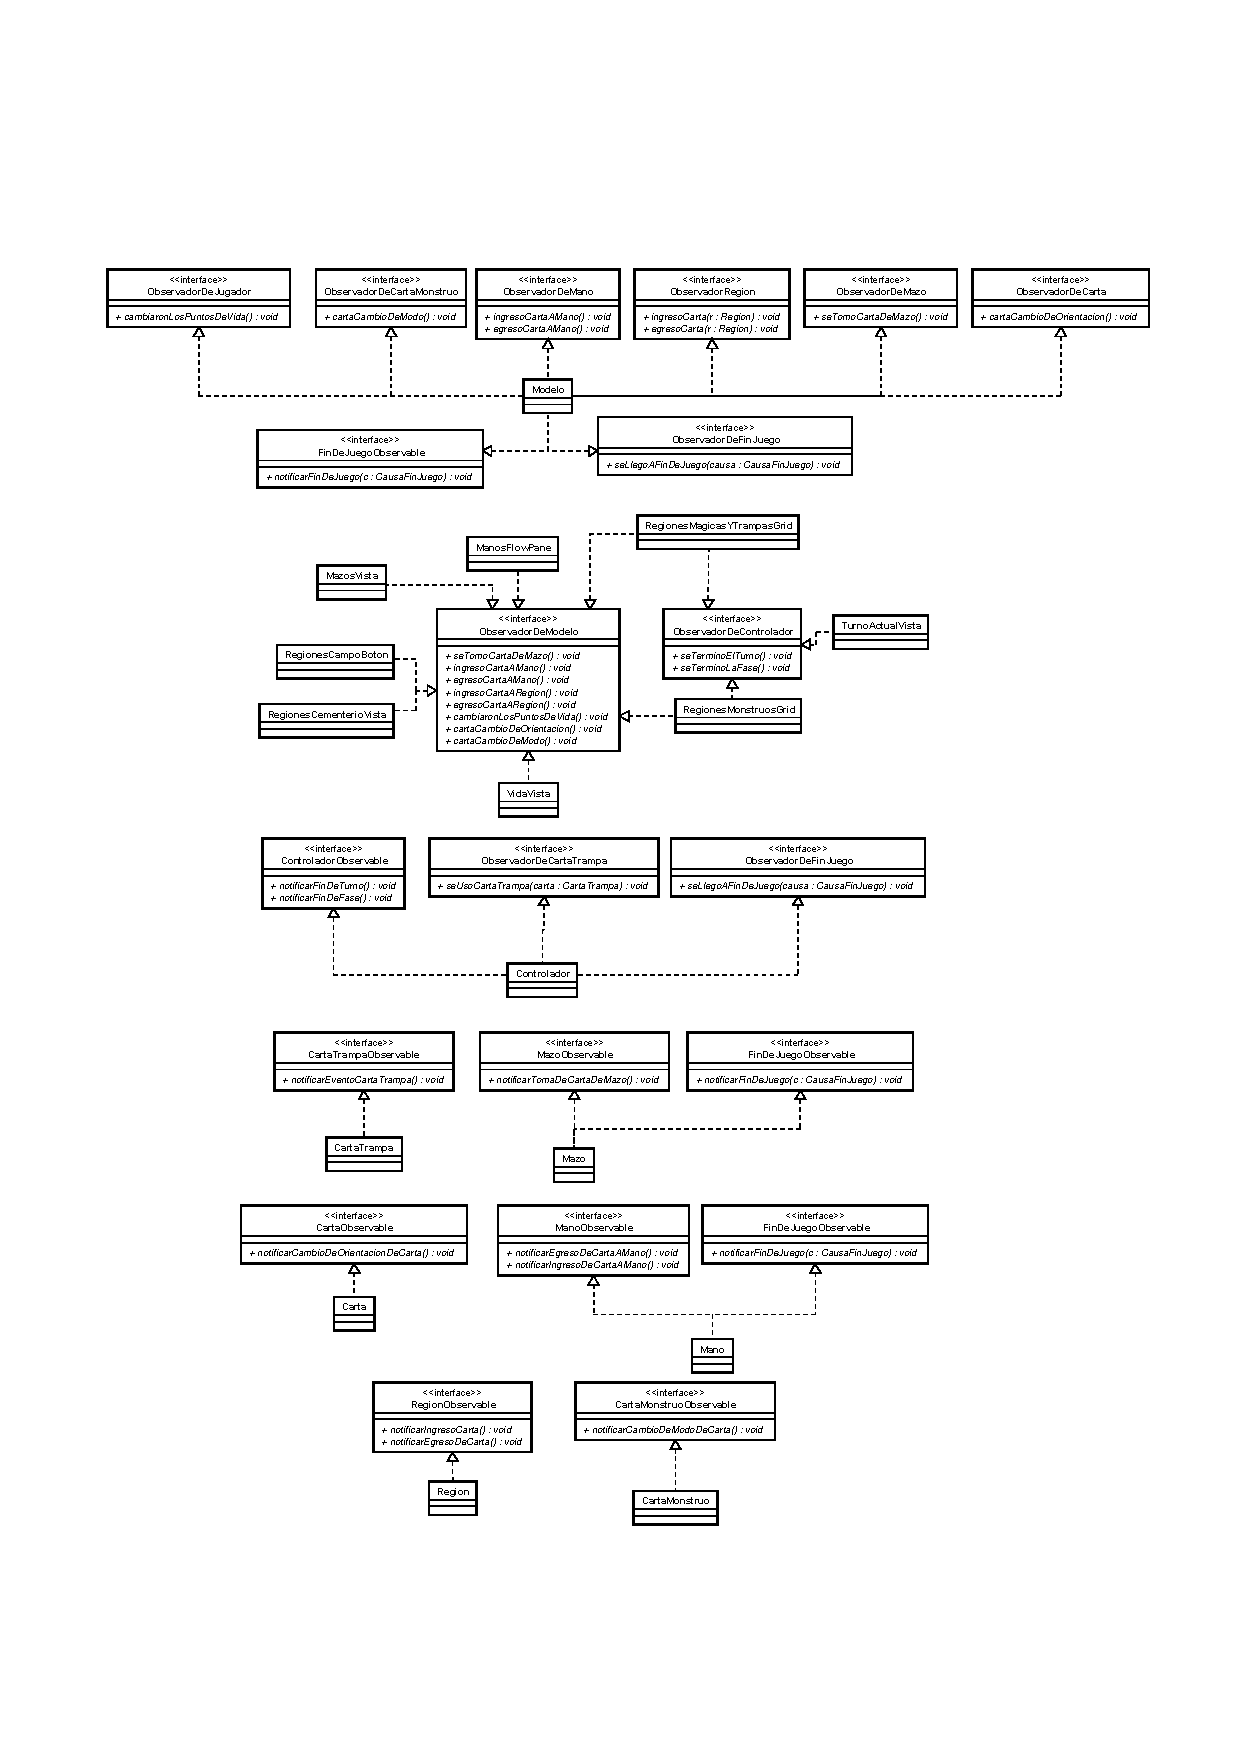
\includegraphics[scale=0.8]{includes/class_Observadores}
	\caption{Observadores}
	\label{class_Observadores}
\end{figure}

Todos implementan registrar y eliminar observador, pero no se los muestra.

\subsection{Jugador}

El diagrama de la figura \ref{}, muestra como se relaciona la clase Jugador con las regiones, con el mazo y con la mano. Ademas, muestra el hecho de que las regiones, el mazo y la mano, contienen cartas. Por otro lado, un jugador, contiene una referencia de otro jugador (oponente).

\begin{figure}[H]
	\centering
	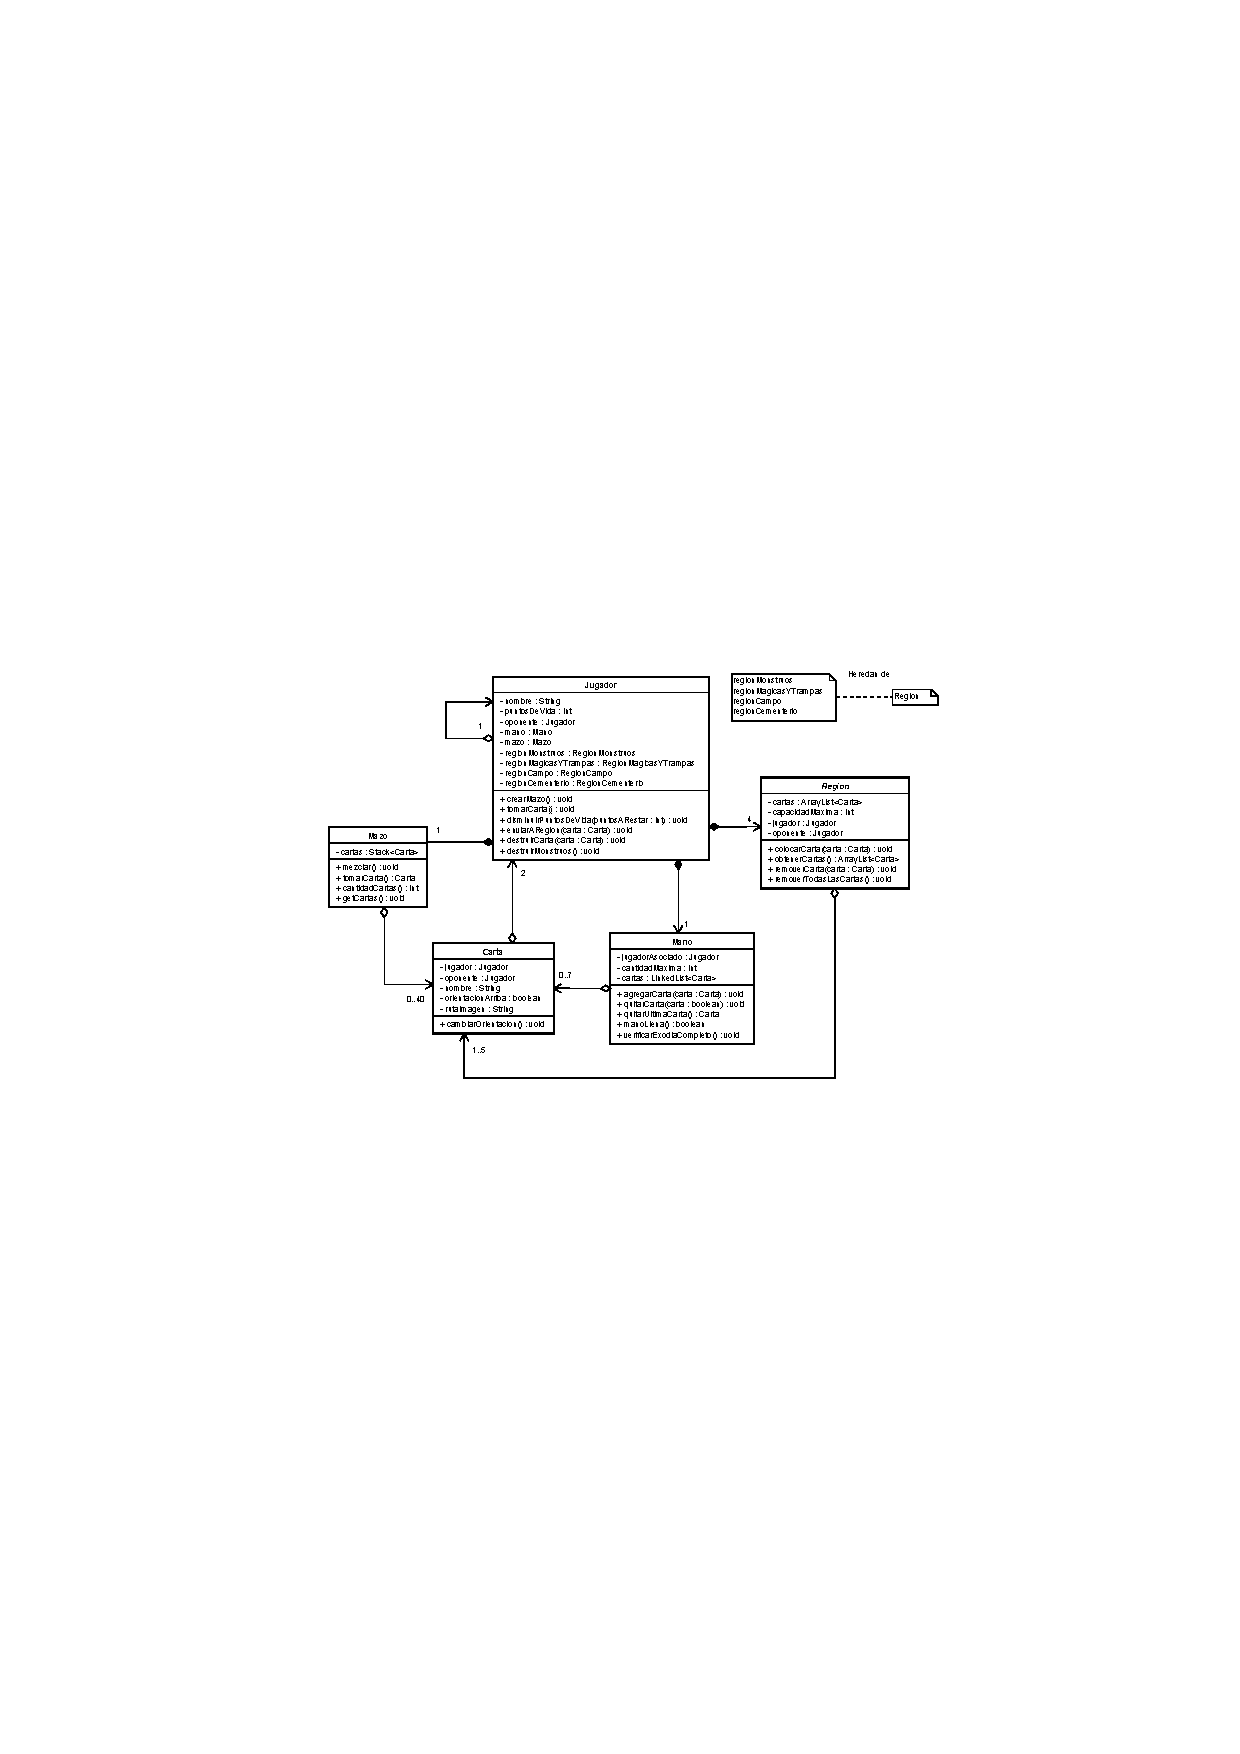
\includegraphics[scale=0.8]{includes/class_Jugador}
	\caption{Jugador}
	\label{class_Jugador}
\end{figure}

\subsection{Carta Monstruo}

\begin{figure}[H]
	\centering
	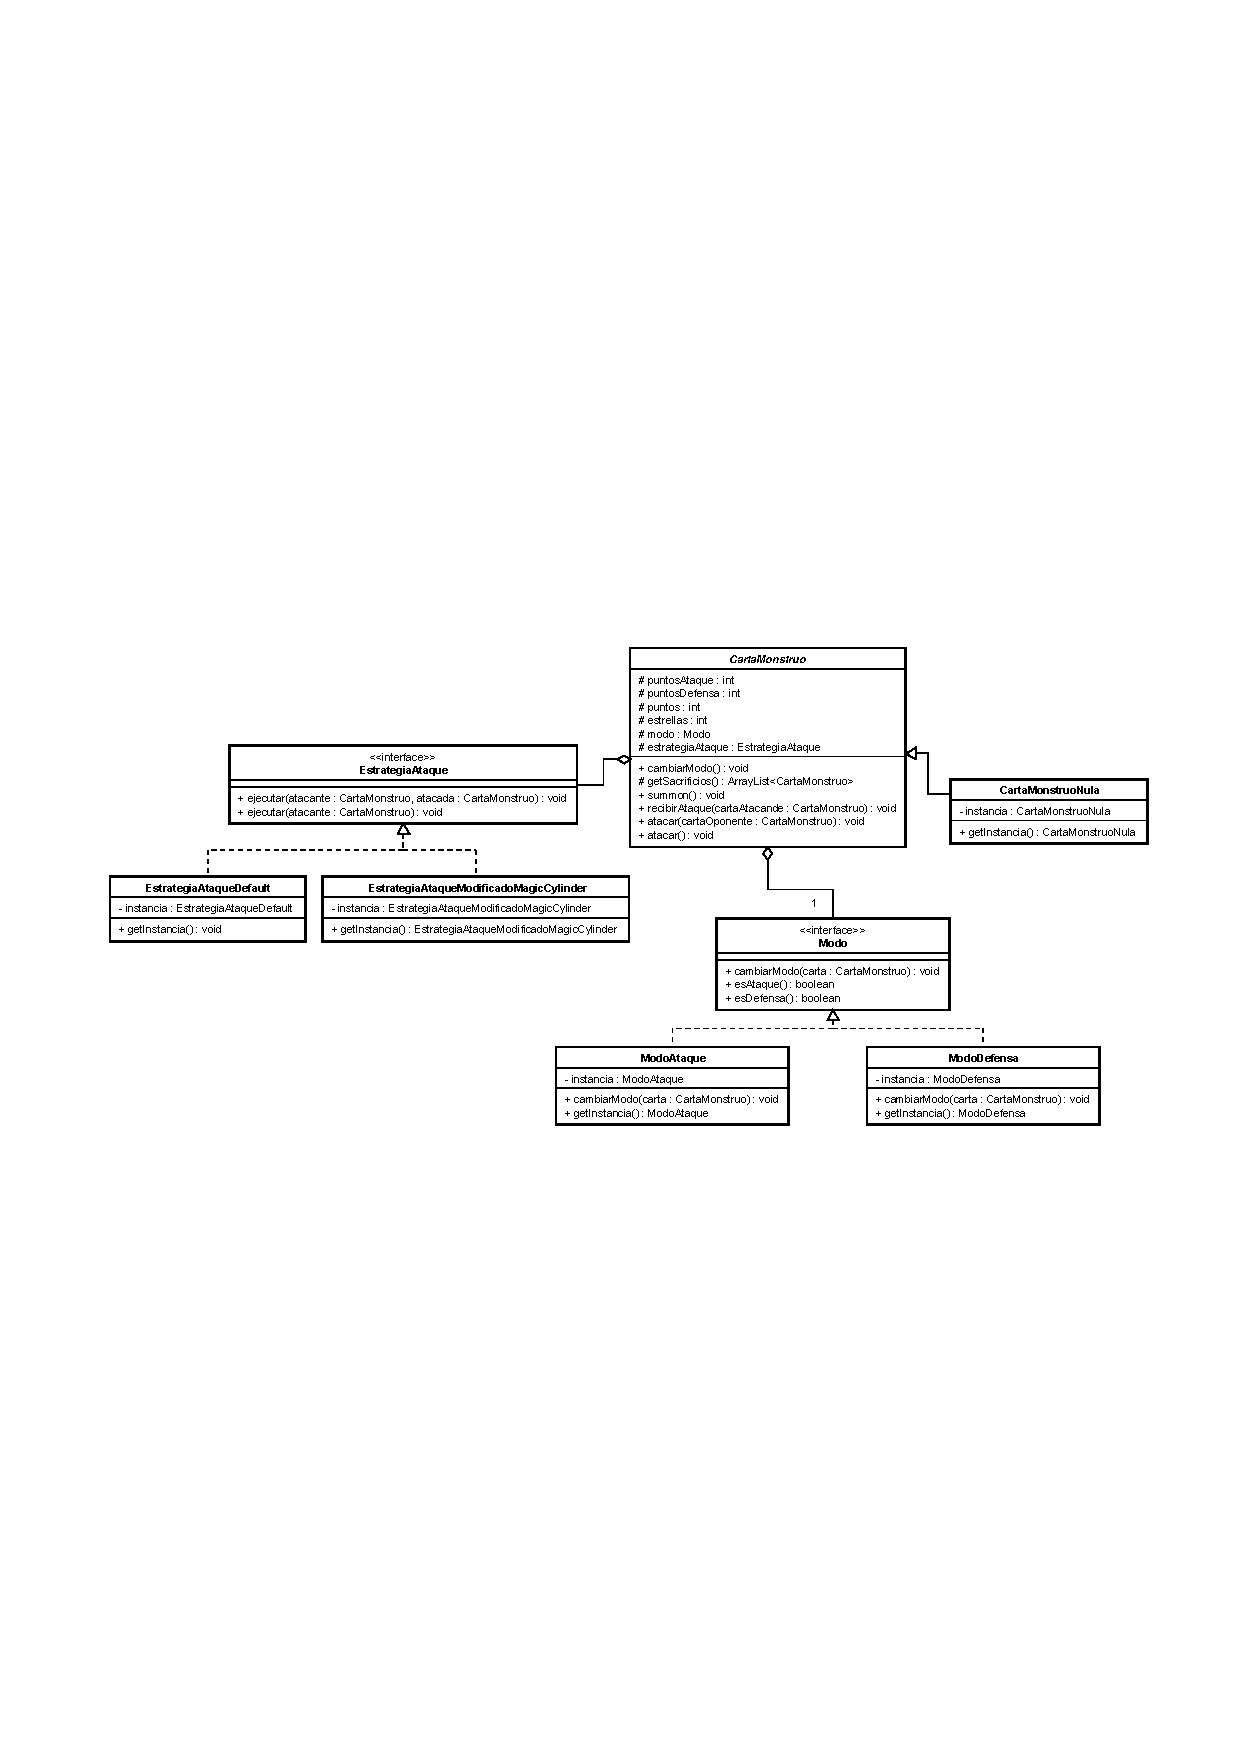
\includegraphics[scale=0.8]{includes/class_CartaMonstruo}
	\caption{Carta Monstruo}
	\label{class_CartaMonstruo}
\end{figure}

\subsection{Controlador}

\begin{figure}[H]
	\centering
	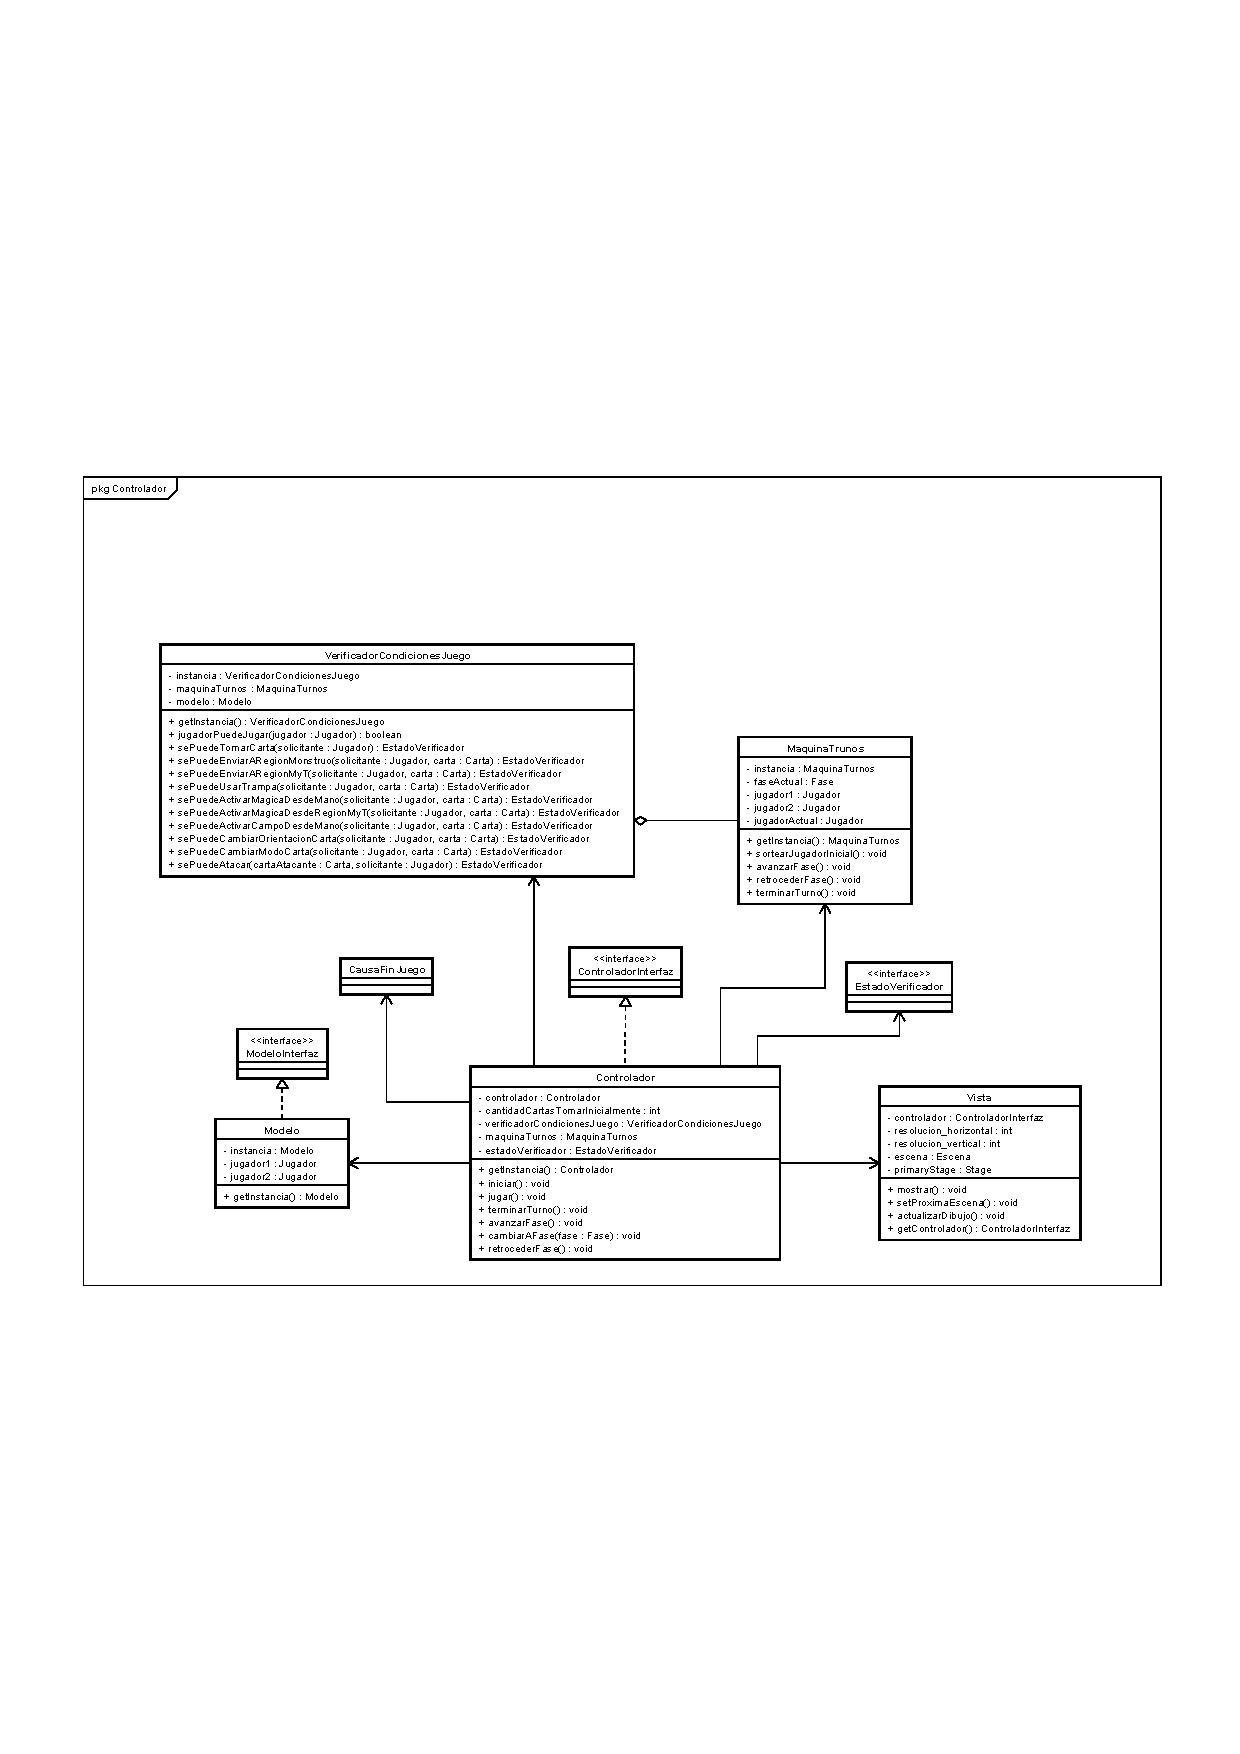
\includegraphics[scale=0.8]{includes/class_Controlador}
	\caption{Controlador}
	\label{class_Controlador}
\end{figure}

\subsection{Fabrica de Cartas}

\begin{figure}[H]
	\centering
	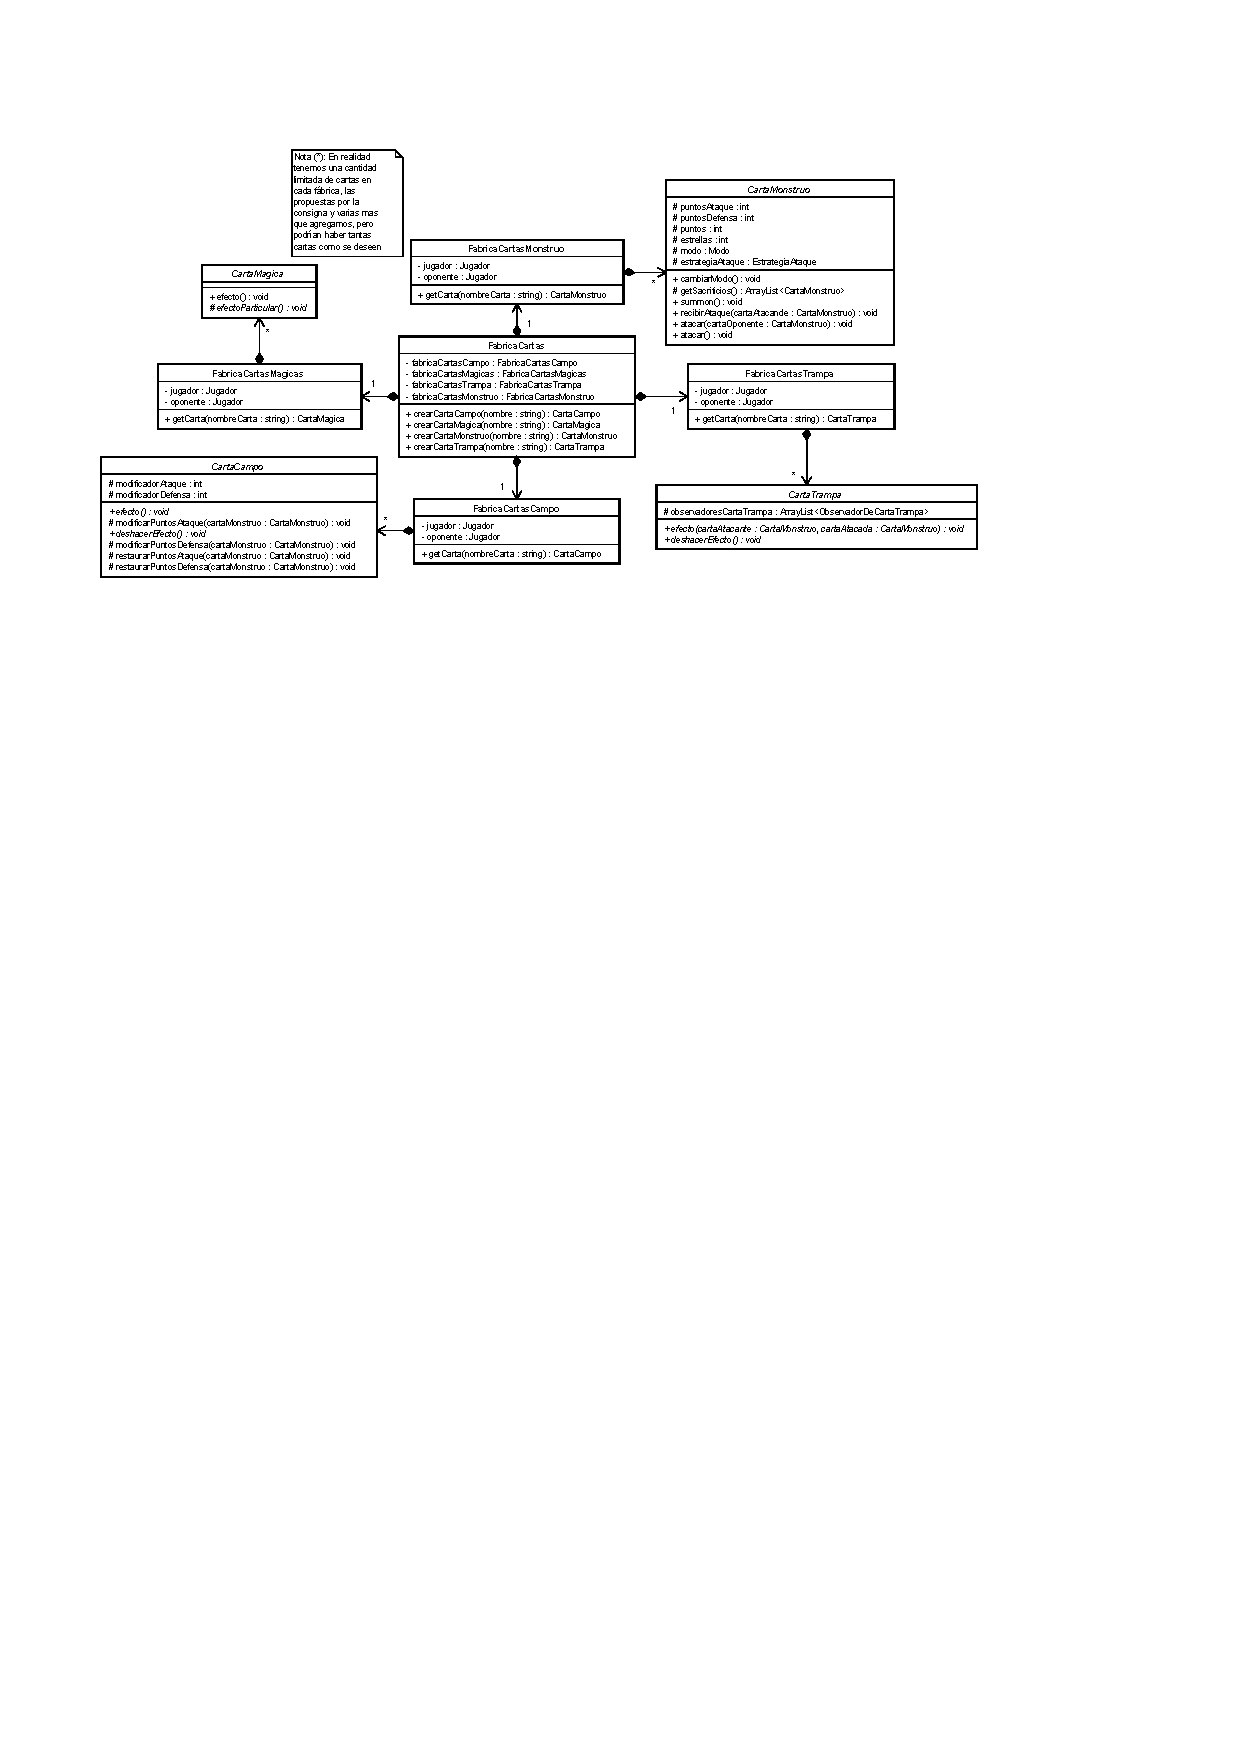
\includegraphics[scale=0.8]{includes/class_FabricaCartas}
	\caption{Fabrica de Cartas}
	\label{class_FabricaCartas}
\end{figure}

\subsection{Regiones}

El diagrama de la figura 4.2, muestra los distintos tipos de regiones posibles, y como estas implementan la interfaz Notificable. La clase Region es abstracta.

\begin{figure}[H]
	\centering
	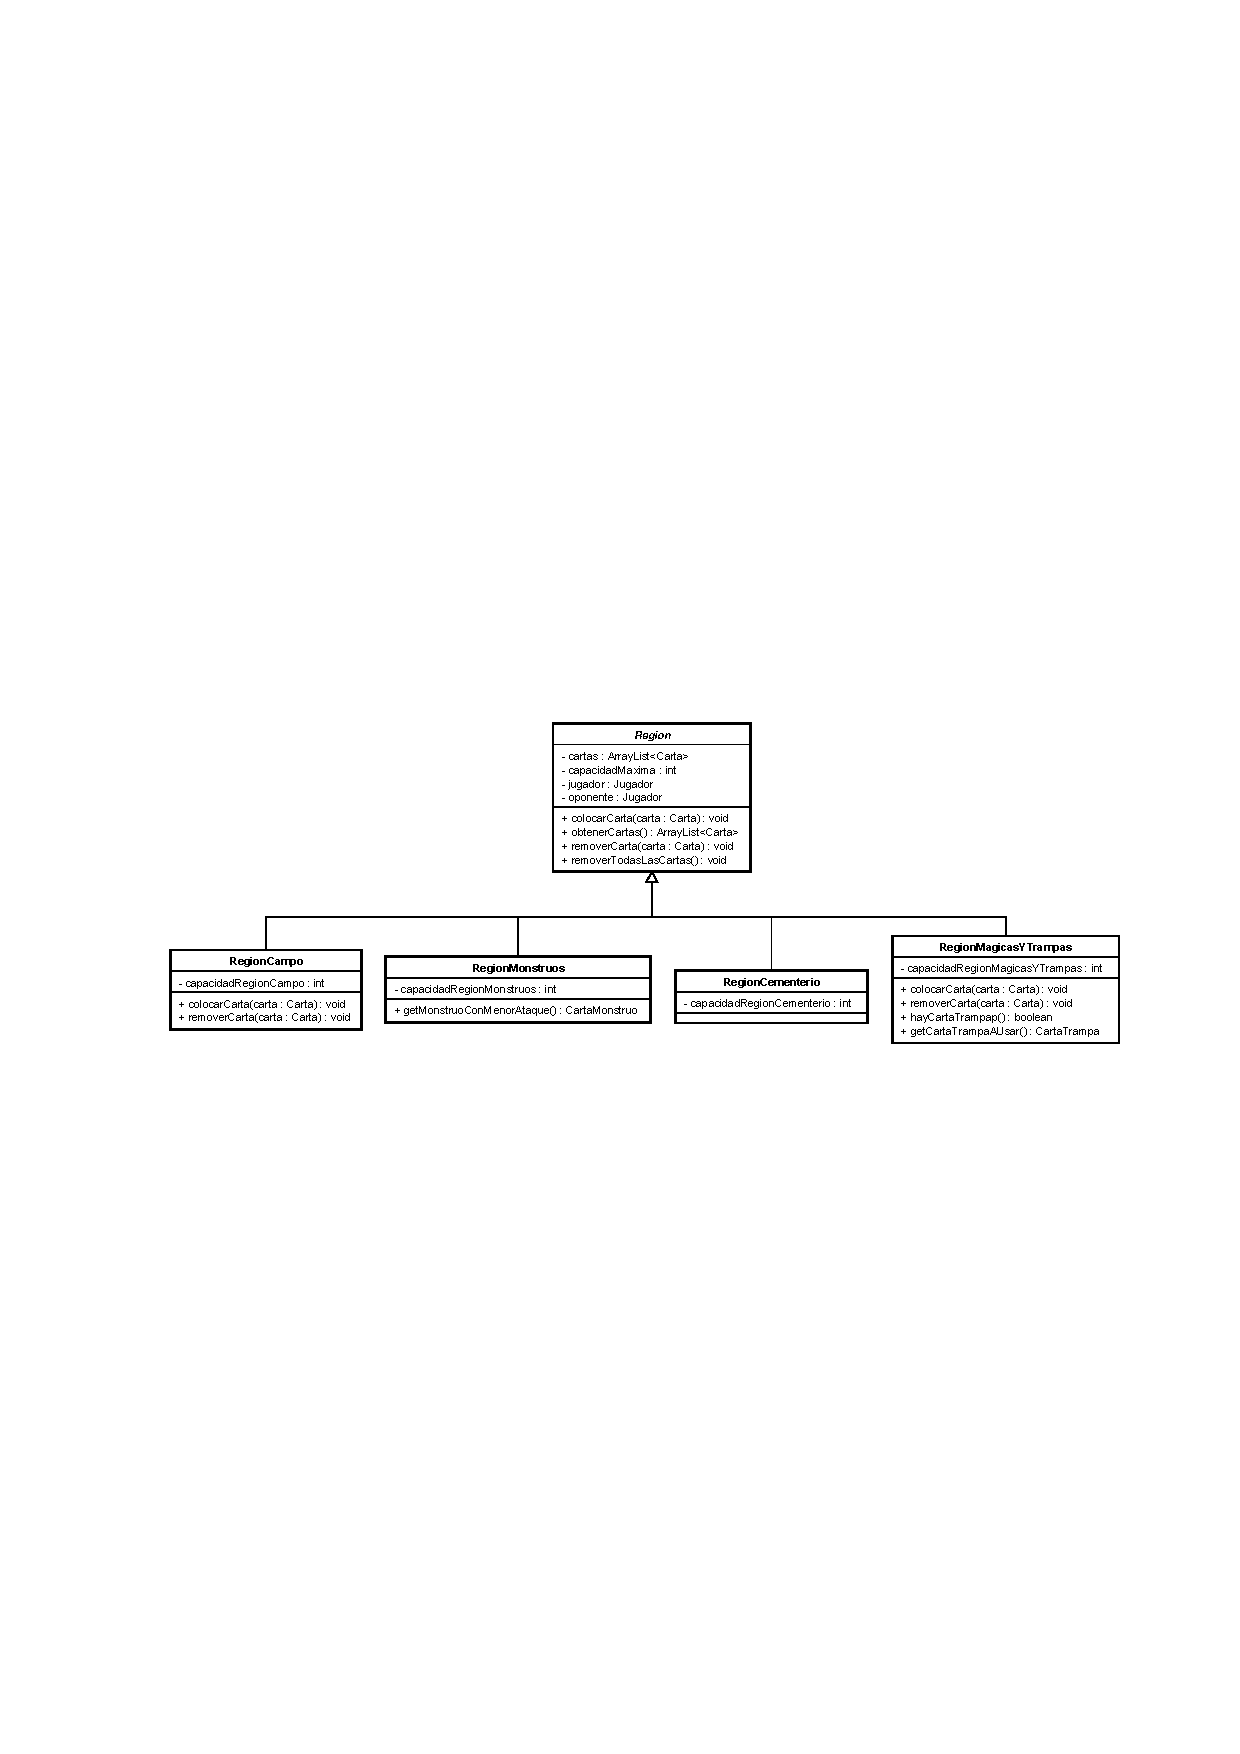
\includegraphics[scale=0.8]{includes/class_Regiones}
	\caption{Regiones}
	\label{class_Regiones}
\end{figure}



\begin{figure}[H]
	\centering
	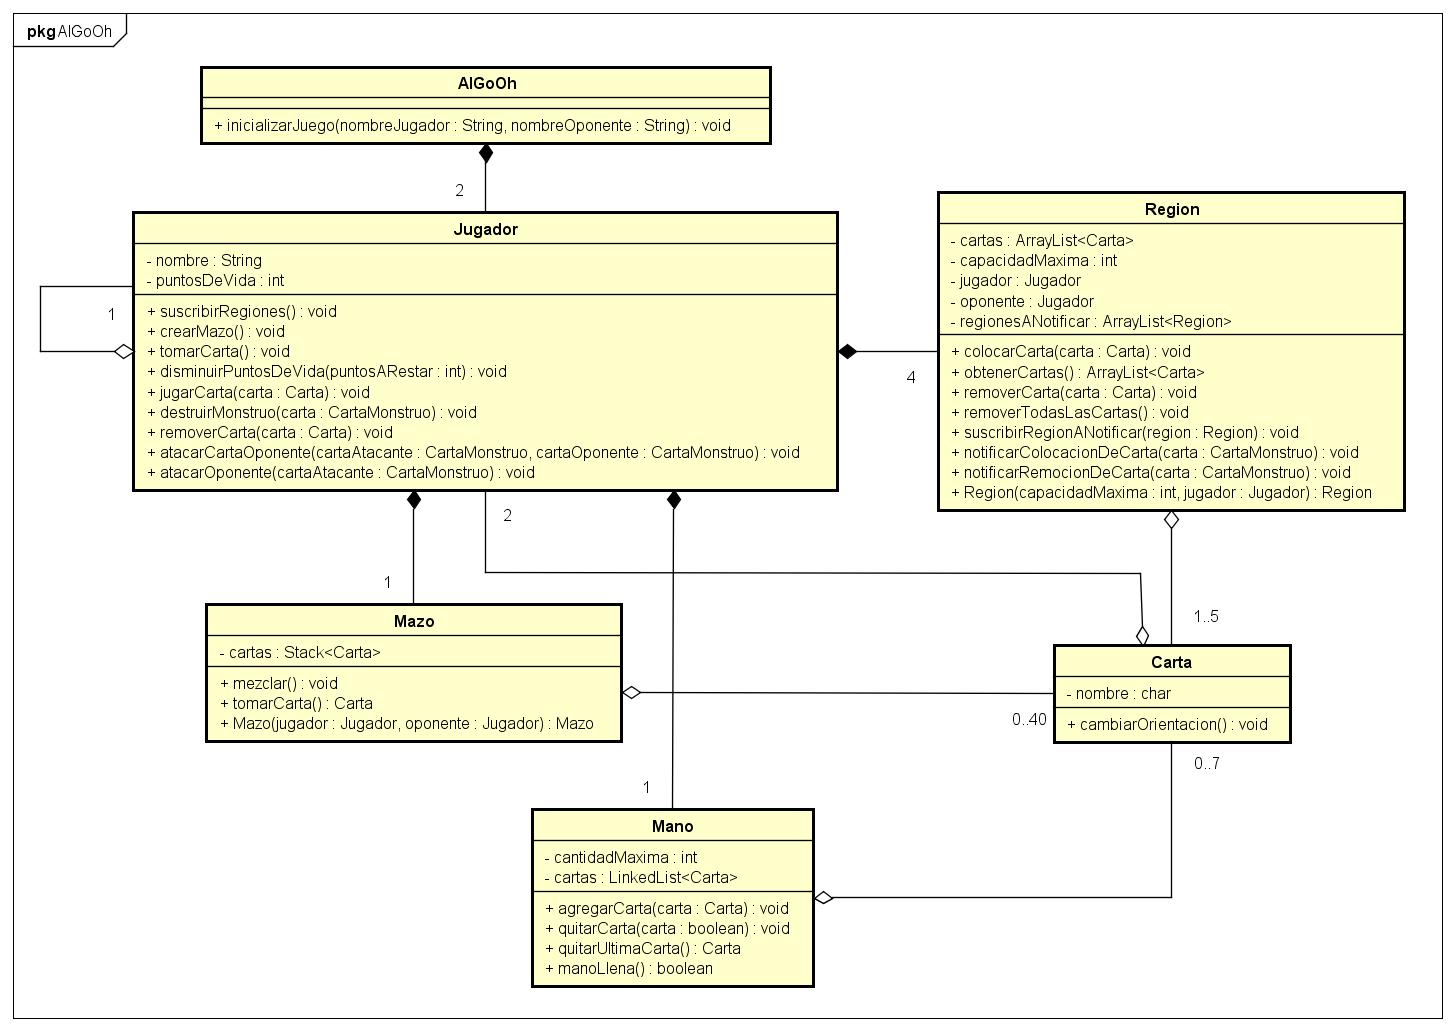
\includegraphics[scale=0.3]{includes/Jugador}
	\caption{Jugador y Carta}
	\label{Jugador}
\end{figure}



\begin{figure}[H]
	\centering
	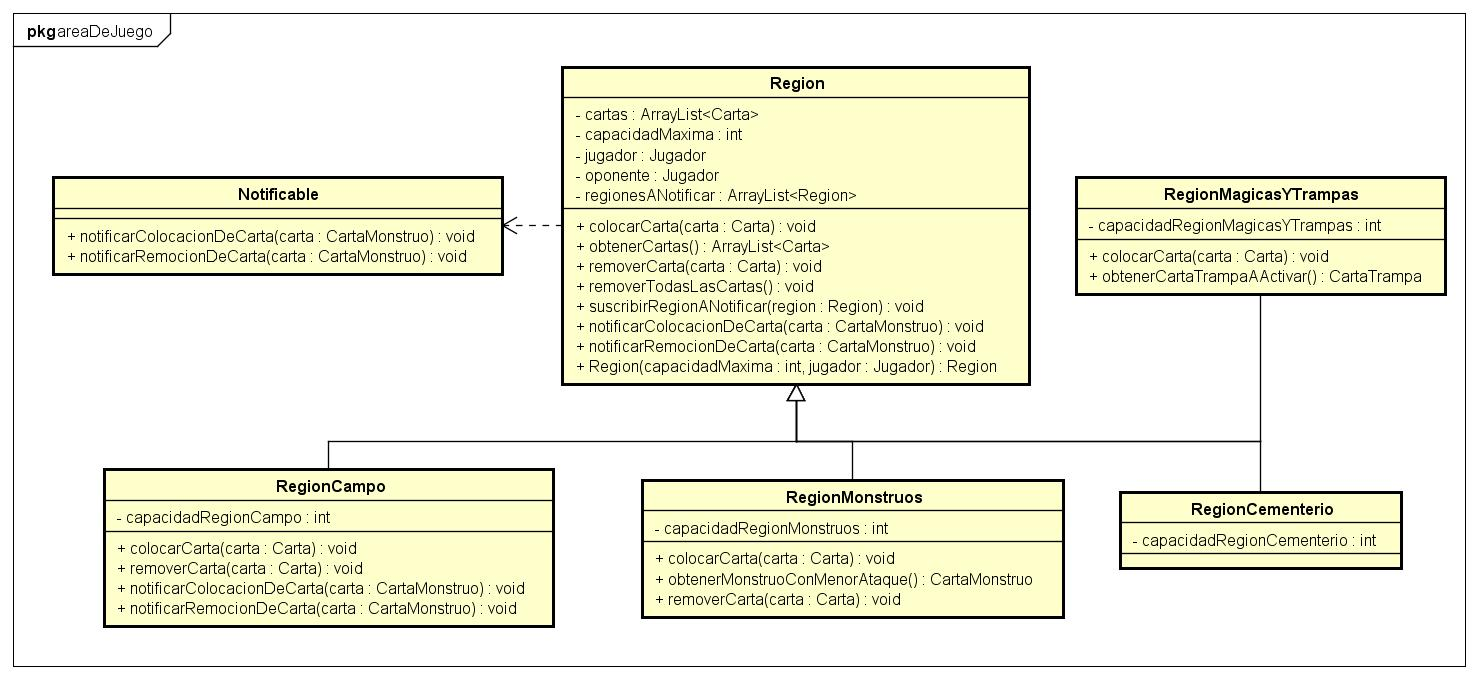
\includegraphics[scale=0.3]{includes/areaDeJuego}
	\caption{Regiones}
	\label{areaDeJuego}
\end{figure}



\begin{figure}[H]
	\centering
	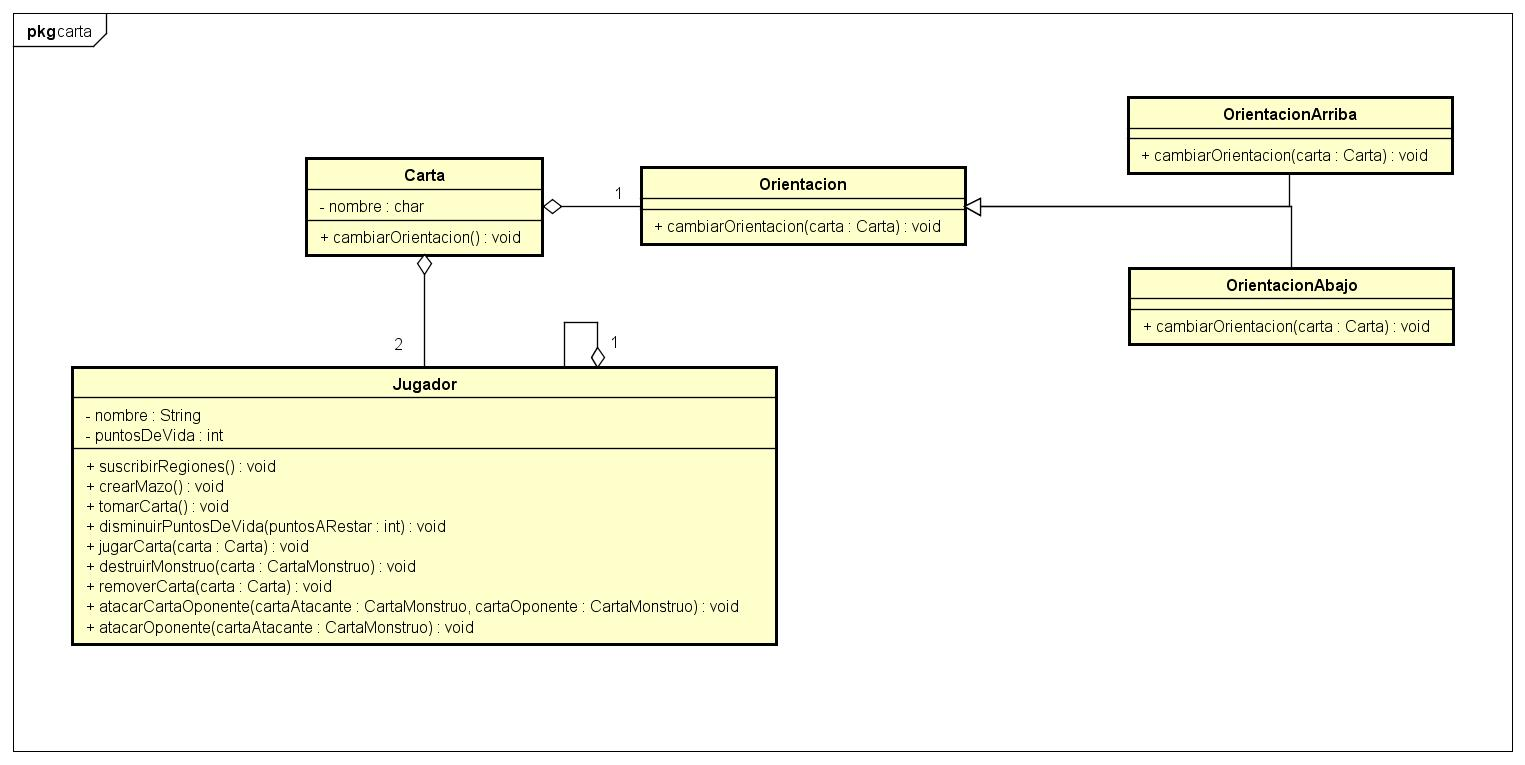
\includegraphics[scale=0.3]{includes/Carta}
	\caption{Carta}
	\label{Cartas}
\end{figure}

El diagrama de la figura 4.4, muestra los distintos tipos de Cartas que puede existir, y tambien el hecho de que existe una fábrica contenedora de cartas.

\begin{figure}[H]
	\centering
	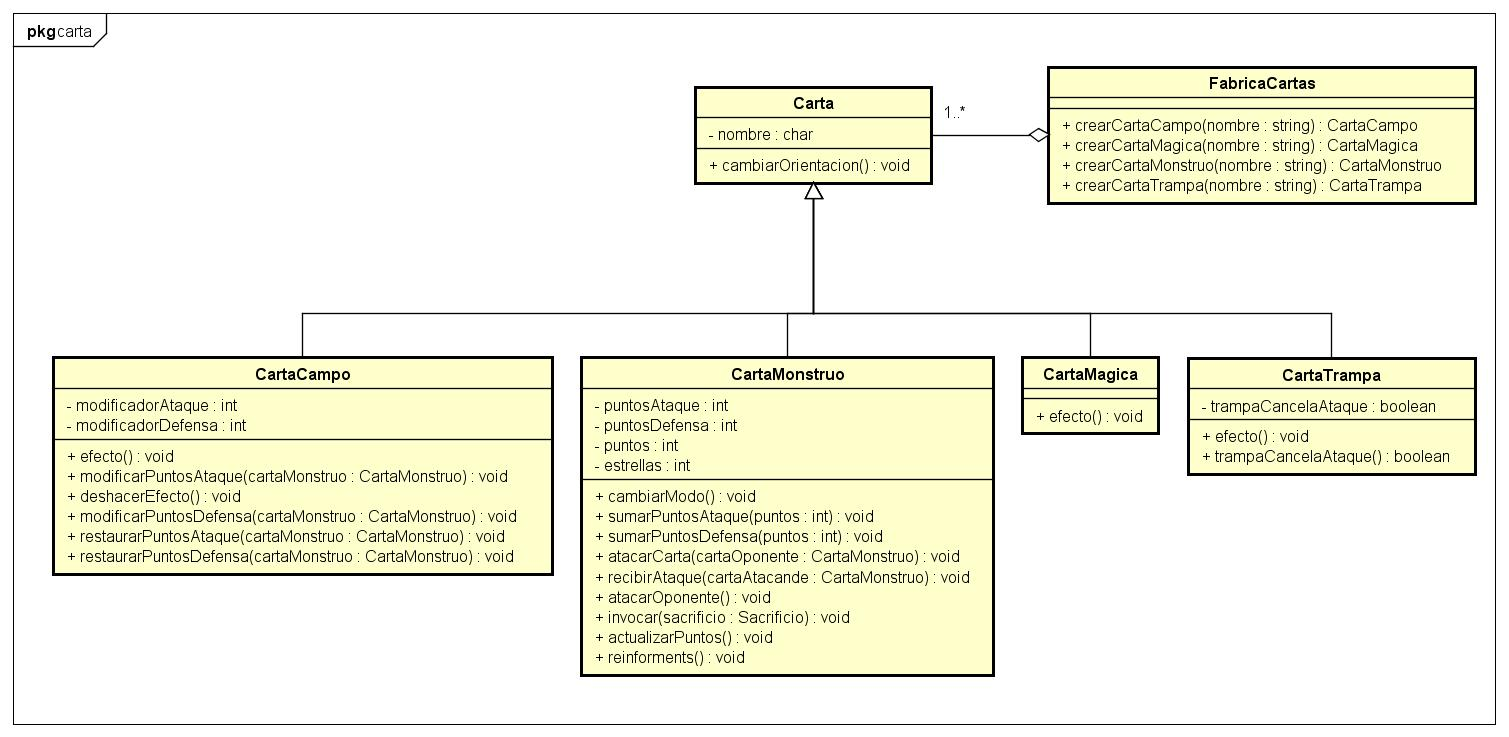
\includegraphics[scale=0.3]{includes/Carta2}
	\caption{Tipos de Cartas}
	\label{TiposCarta}
\end{figure}

El diagrama de la figura 4.5 muestra a la clase abstracta CartaMonstruo. La misma contiene un modo, y por otra parte, tendra como hijos a todos los monstruos. La clase sacrificio, conoce a las cartas monstruos gracias al jugador (que es el que decide que sacrificar) y ademas las contiene, 


\begin{figure}[H]
	\centering
	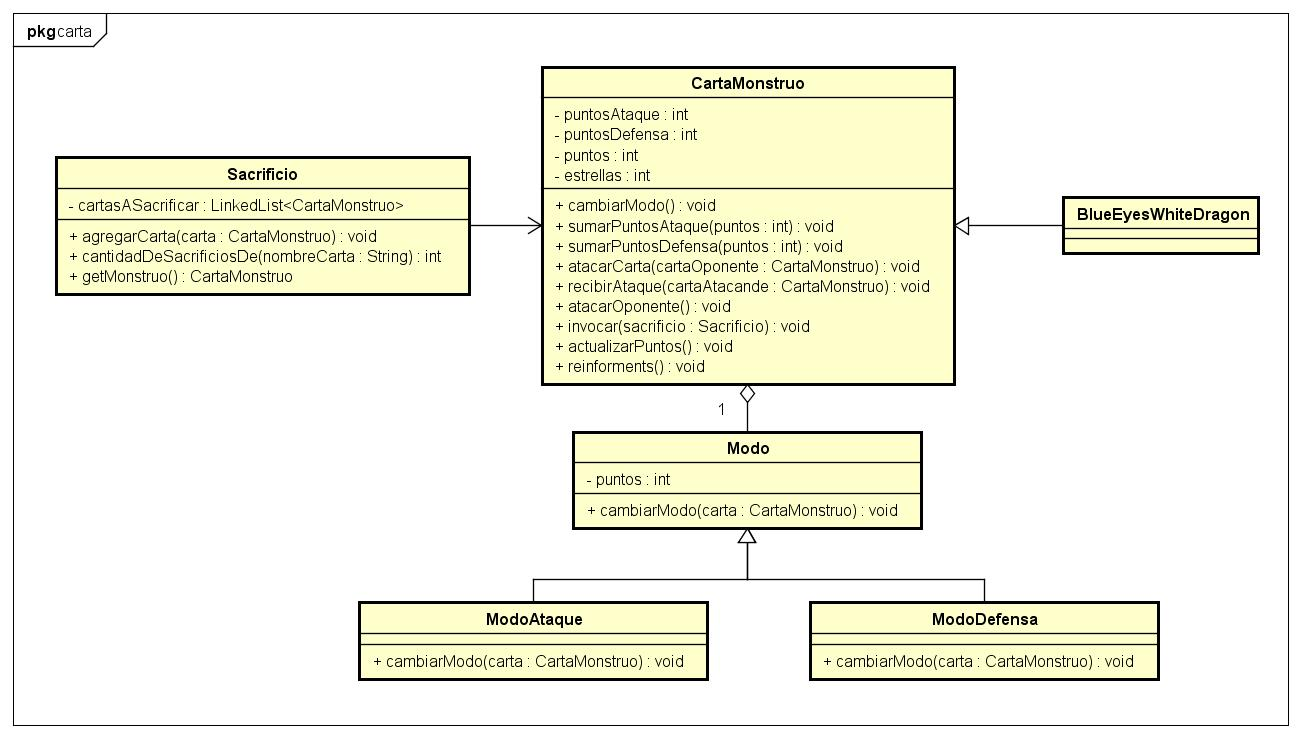
\includegraphics[scale=0.3]{includes/CartaMonstruo}
	\caption{Carta Monstruo}
	\label{CartaMonstruo}
\end{figure}

El diagrama de la figura 4.6 muestra las fábricas de cartas.

\begin{figure}[H]
	\centering
	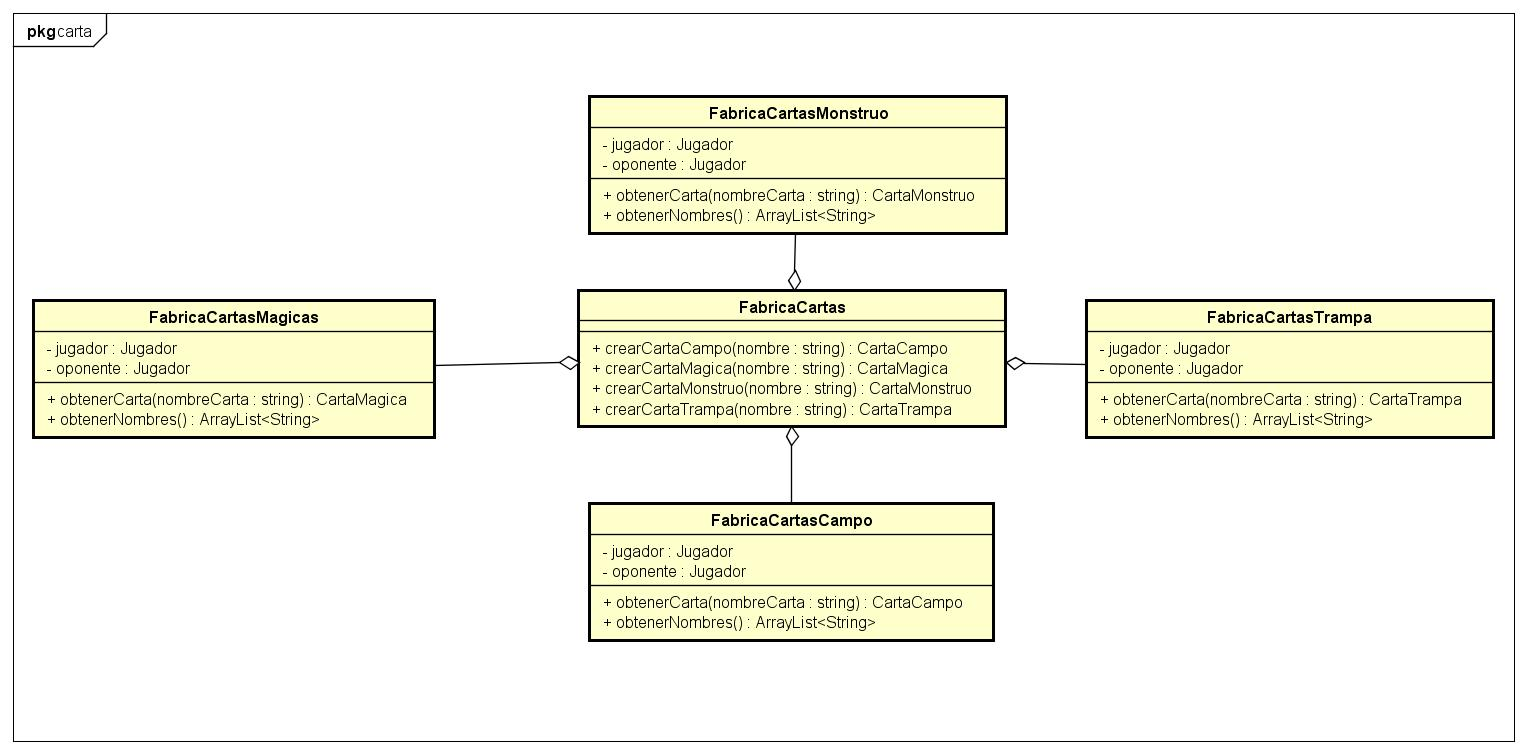
\includegraphics[scale=0.3]{includes/Fabricas}
	\caption{Fabricas}
	\label{Fabricas}
\end{figure}

\clearpage
\section{Diagramas de secuencia}

[ Varios diagramas de secuencia, mostrando la relación dinámica entre las
clases planteando una gran cantidad de escenarios que contemplen las
situaciones del trabajo práctico]

\begin{figure}[H]
	\centering
	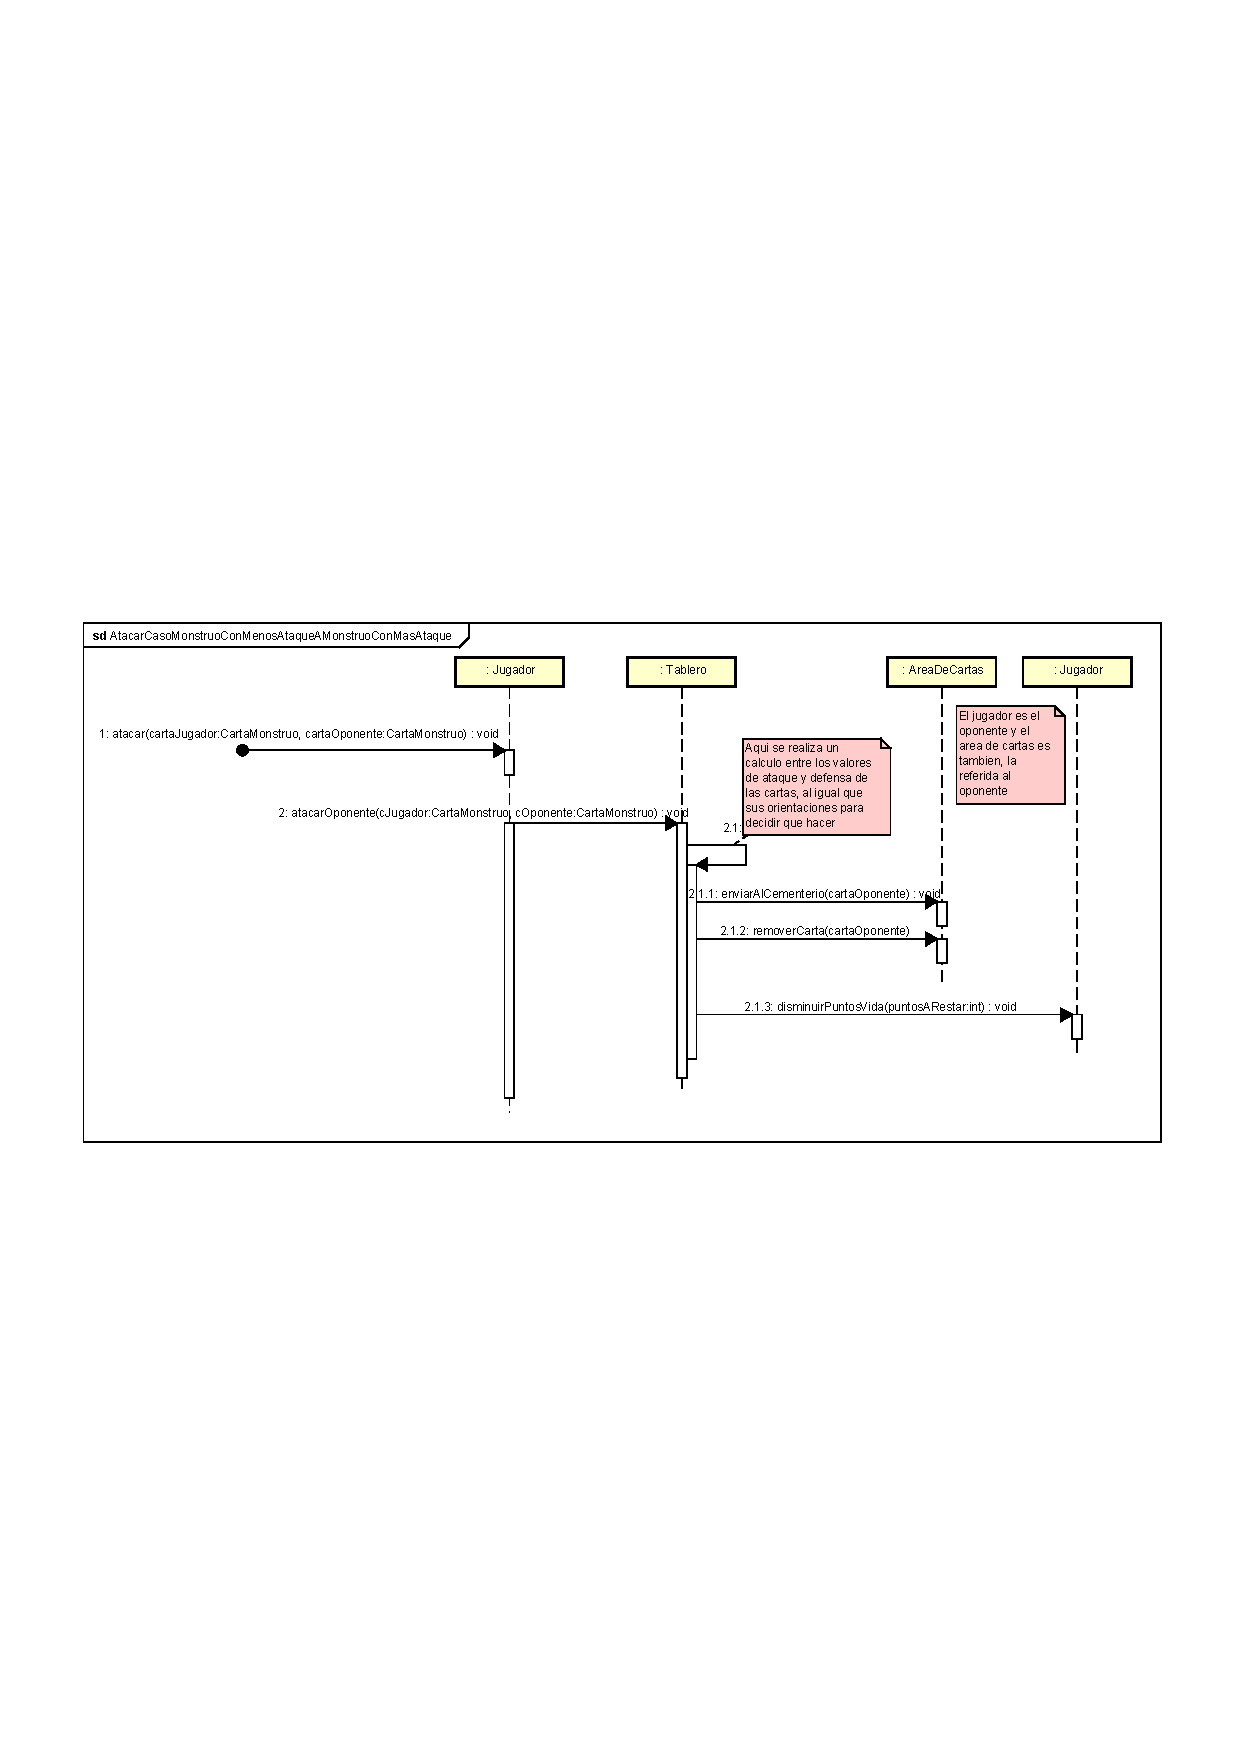
\includegraphics[scale=0.9]{includes/AtacarCasoMonstruoConMenosAtaqueAMonstruoConMasAtaque}
	\caption{titulo.}
	\label{AtacarCasoMonstruoConMenosAtaqueAMonstruoConMasAtaque}
\end{figure}
\begin{figure}[H]
	\centering
	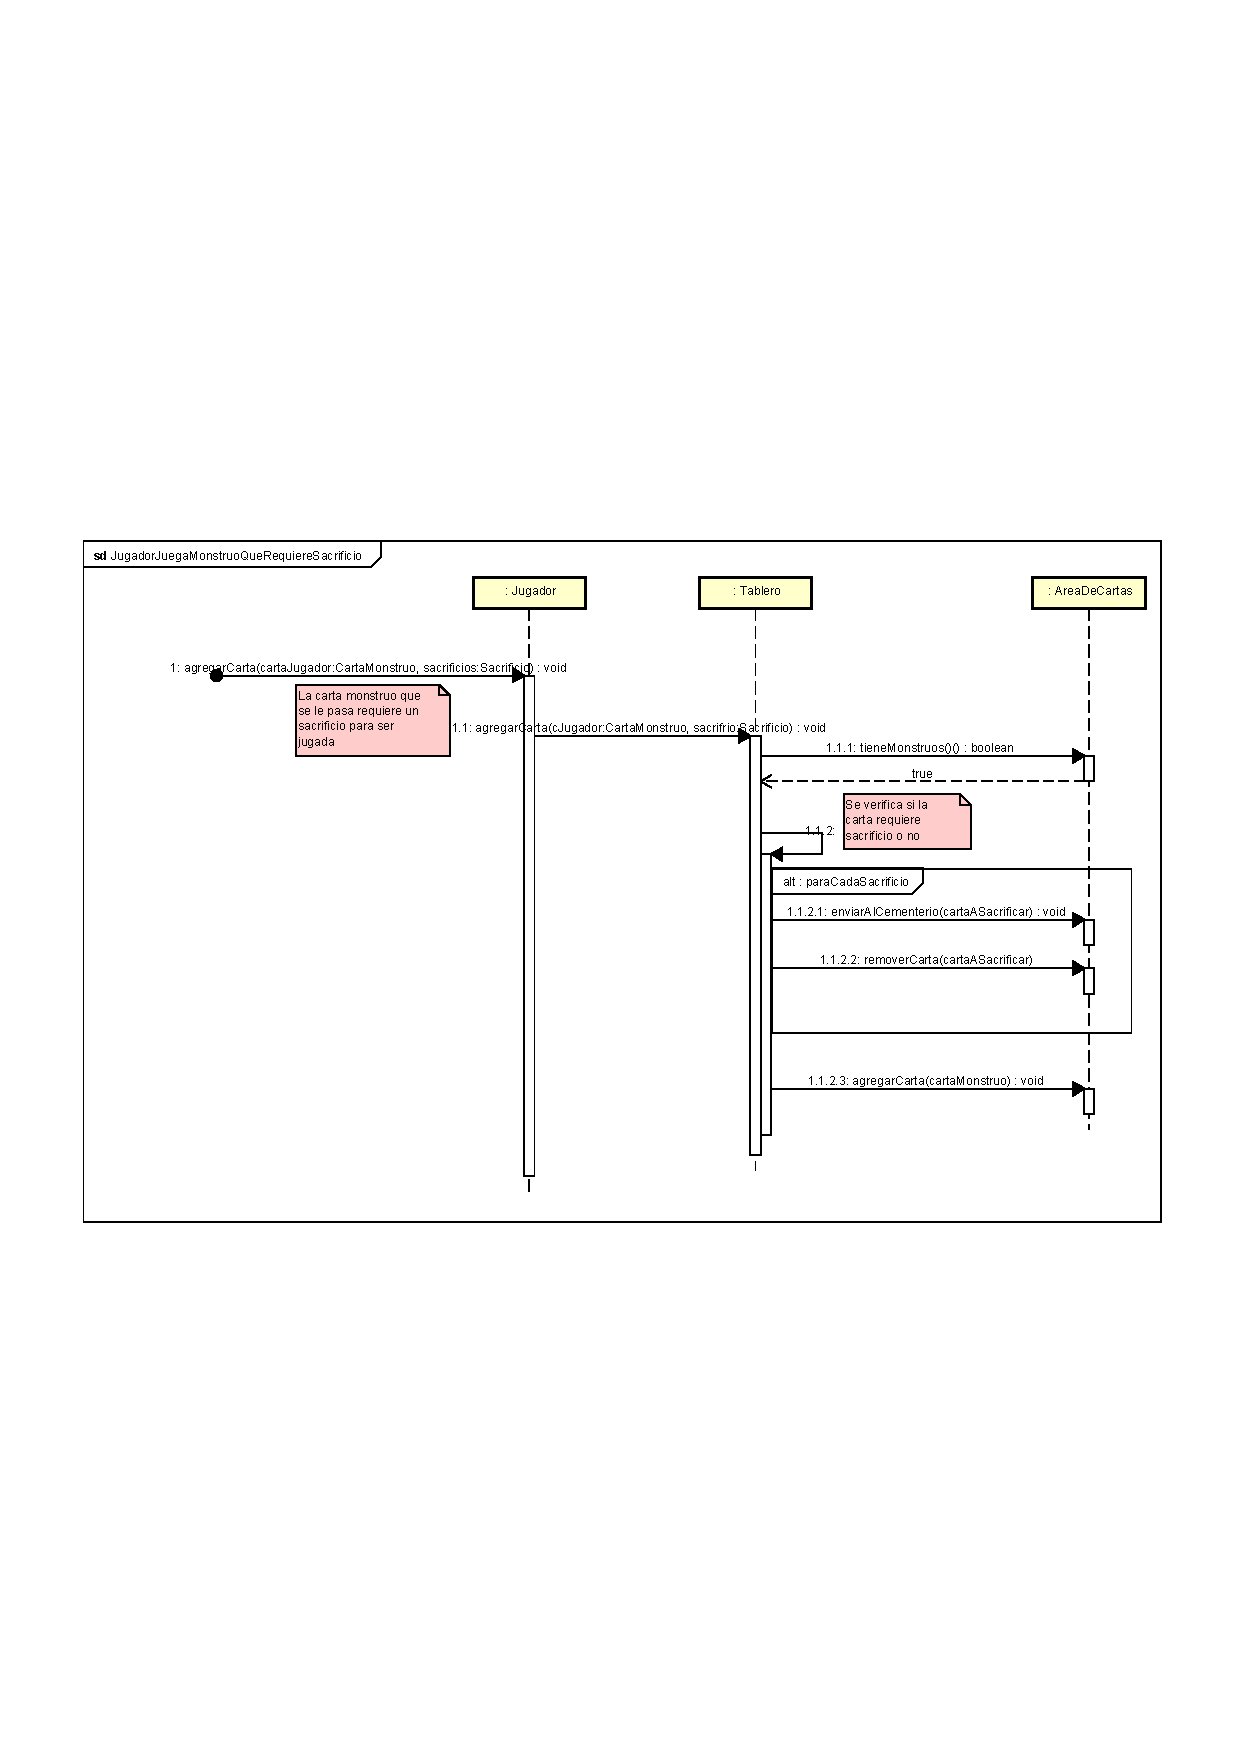
\includegraphics[scale=0.9]{includes/JugadorJuegaMonstruoQueRequiereSacrificio}
	\caption{titulo.}
	\label{JugadorJuegaMonstruoQueRequiereSacrificio}
\end{figure}
\begin{figure}[H]
	\centering
	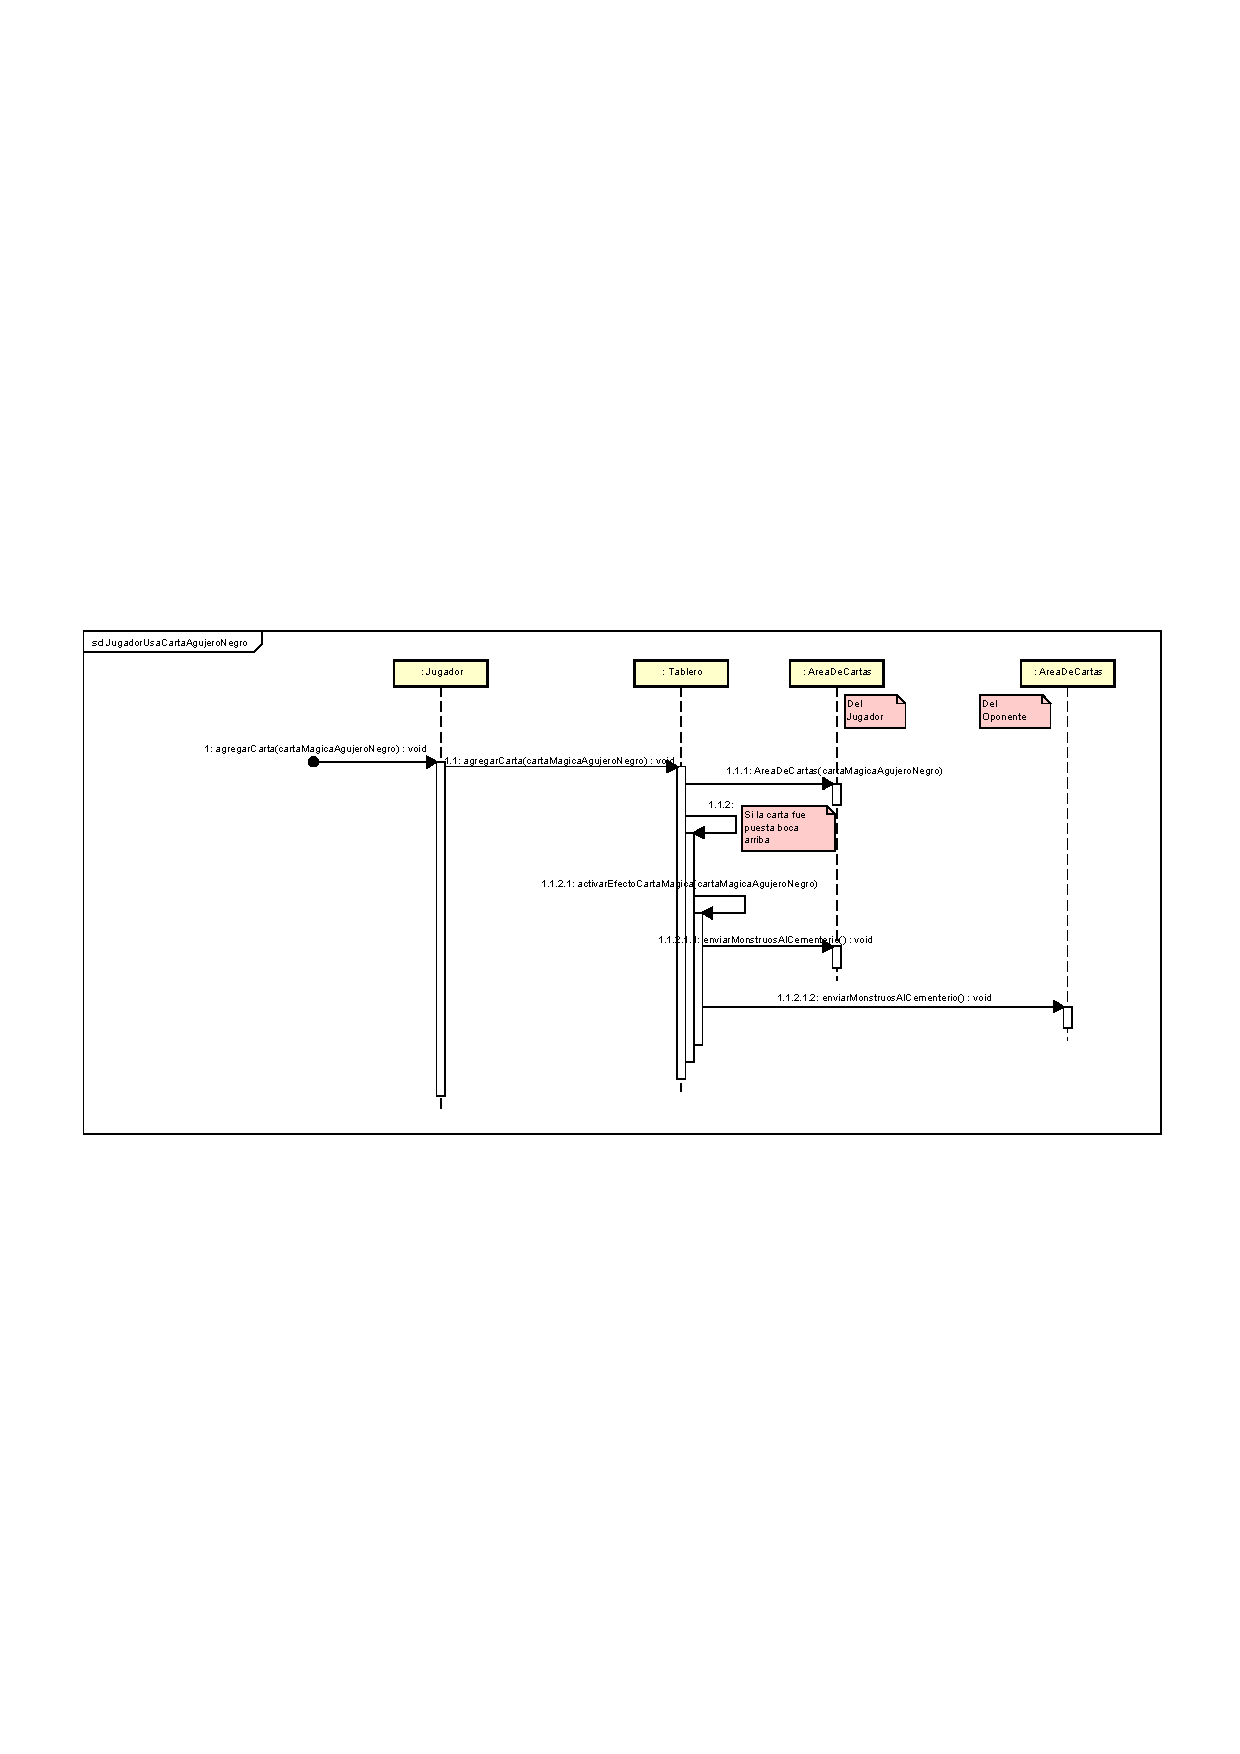
\includegraphics[scale=0.9]{includes/JugadorUsaCartaAgujeroNegro}
	\caption{titulo.}
	\label{JugadorUsaCartaAgujeroNegro}
\end{figure}

\section{Diagramas de paquetes}

[incluir un diagrama de paquetes para mostrar el acoplamiento de su
trabajo ]

\section{Diagramas de estado}

[Incluir diagramas de estados, mostrando tanto los estados como las
distintas transiciones de los mismos para varias entidades del trabajo
práctico ]

\section{Detalles de implementación}
[Explicar los elementos más relevantes del diseño. Es decir: qué
entidades se han creado, qué responsabilidades tienen asignadas, cómo
se relacionan, etc]




{\large\textbf{Progreso}}

\bigskip


Para hacer este trabajo práctico, utilizamos TDD para el desarrollo y, durante las dos primeras entregas, usamos como táctica de programación Pair Programming para avanzar con el modelo, con reuniones físicas o varias veces, por videoconferencia. Ya llegando al final del trabajo práctico, cuando tuvimos que implementar el MVC, dividimos las tareas en el armado de la vista, controlador, modelo e informe. 

\bigskip


{\large\textbf{Refactorizaciones}}

\bigskip

Para la realización de este trabajo práctico, nuestro modelo fue cambiando en reiteradas ocasiones e implementamos múltiples refactorizaciones. 

\medskip

En un principio, habiamos decidido en conjunto que lo ideal era no utilizar un tablero y buscamos lograr la interacción entre los dos jugadores. A medida que fuimos avanzando en la primera entrega, tuvimos complicaciones en reiteradas ocaciones y terminamos optando por utilizar el tablero, lo que nos hacía creer que todo era mas fácil. Completamos la entrega y el profesor nos ayudó y nos hizo ver que la utilización de un tablero como entidad arbitraria, no era lo mejor teniendo en cuenta el paradigma orientado a objetos. Cada objeto del juego debería comunicarse con otro para representar en mayor proporción la realidad, y no crear un arbitro que no existe. Esto rompería con el \textbf{Principio SOLID de Responsabilidad Única} (el tablero estaría encargado de todas las acciones) y además, con el \textbf{Principio de Inversión de la Dependencia}, ya que todos dependerían de esta entidad.

\medskip

Entonces, retomamos la idea de que los dos jugadores se relacionen e interactuen entre ellos. Refactorizamos para lograr eliminar el tablero, y en ese momento habíamos decidido que el ataque lo haga el jugador utilizando la carta y no que sea la carta la que atacaba al oponente. Esto tambien lo hablamos con el profesor y tomamos la decisión de que cada carta sea la que realiza el ataque y además, los efectos tambien sean implementados por cada carta. La implementación del efecto, en principio, la realizamos con una interfaz que obligaba a que todos tengan un efecto pero, como cada efecto era muy particular (recibia parametros distintos) optamos por hacer que cada clase que use efecto tenga su método diferente al resto.


\medskip


Otro asunto que nos obligo a refactorizar, fueron los sacrificios. Lo que hicimos en primer lugar, fue hacer un simple array que contenía los monstruos a sacrificar, para luego terminar creando una entidad sacrificio la cual contiene los monstruos que el usuario decide sacrificar y en el momento de la invocacion se envian al cementerio.

\medskip

Mientras desarrollabamos la segunda entrega, vimos la necesidad refactorizar nuevamente y convertir a cada tipo de carta en una clase abstracta, para que los monstruos especificos hereden de ellas y estos sean los que tengan las particularidades de cada una. Esto cumple a la perfección con el \textbf{Principio de Sustitución de Liskov}, donde todas las clases hijas (Monstruos) son cartas monstruo y las cartas monstruo, son cartas. Esto aplica para toda la relación de cartas, y cumple el principio ya que todas las clases hijas se pueden ubicar en lugar de la clase padre. 

\medskip

También refactorizamos el calculo de daño y ya no son las cartas monstruos las que restaban puntos al jugador, sino que el jugador se quita sus propios puntos de vida (Cumple con principio SOLID abierto/cerrado, la clase debe estar cerrada al exterior para su modificación, pero abierta para su extención.)

\medskip

Ya preparando la entrega final, volvimos a aplicar una refactorización que consistía en que el jugador (que hasta entonces, era el encargado de atacar y de llevar a cabo las tareas) ya no sería el encargado de implementar las estrategias de las cartas, sino que ahora ellas mismas son las que atacan y activan sus efectos. Esta refactorización, también cumple con el \textbf{Principio de Responsabilidad Única} (el jugador, da ordenes a las cartas pero no le interesa como las cumplen) 

\medskip

Una vez finalizado el modelo, comenzamos a implementar la interfaz gráfica y en principio, nuestra idea fue conectarla directamente con el modelo pero nos dimos cuenta de que el usuario iba a interactuar con mas de lo que debía. Esto rompe con el \textbf{Principio de Segregación de la Interfaz} (el cliente solo debe conocer lo que usa) y hablamos con el profesor para solucionar esto. Su recomendación fue utilizar el Patron de Diseño MVC para interactuar con el usuario.

 \bigskip

A continuación se listan los patrones de diseño utilizados, junto con las explicaciones de para que fueron usados.

 \bigskip

\begin{description}

\item[MVC] Como lo indica el nombre, utilizamos este patrón para la relación entre el Modelo, la Vista y el Controlador. -- Falta explicar y ver como lo hacemos --

\item[Observer] La vista, se encarga de observar al modelo y cada parte importante del mismo, implementa la interfaz Observable. Estos objetos observables notifican a las vistas de cambios en su comportamiento. 

\item[Factory] Utilizamos este patrón de diseño para la generación de cartas de cualquier tipo, por lo que creamos 4 fábricas (cartas mágicas, cartas trampas, cartas monstruo, cartas campo).

\item[State] Este patrón de diseño, lo utilizamos para especificar que, una carta, puede estar boca arriba o boca abajo y cambiar su estado en cualquier momento con un simple llamado. Tambien, las cartas monstruos, pueden cambiar de modo de ataque a modo de defensa y asi cambiar su estado cuando el jugador lo desee. Dependiendo del estado en el que este la carta, las acciones a realizar serán distintas.  

\item[Patron 5] Hablar cual mas hay.

\end{description}





\section{Excepciones}

[Explicar las excepciones creadas, con qué fin fueron creadas y cómo y
dónde se las atrapa explicando qué acciones se toman al respecto una vez
capturadas.]

\bigskip

{\large \raggedright \textbf{Controlador}}

\begin{description}


\item[NoEsUnaCartaParaAtacar] La carta no puede realizar ataques.

\item[CartaNoPuedeCambiarOrientacionEnTurnoActual] Su nombre lo indica a la perfección.

\item[CartaYaAtacoEnTurnoActualError] En caso de que ya se haya realizado un ataque con esa carta.

\item[JugadorNoPermitidoParaJugarError] El jugador quiere jugar en el turno del enemigo.

\item[NoEsFaseX] Existe una excepción de este tipo para cada fase con el fin de evitar que se realizen acciones indebidas para el tipo de fase.

\item[NoHayEspacioLibreEnRegionMyT] La carta no se puede colocar si la región esta llena.

\item[NoHayEspacioLibreEnRegionMonstruo] La carta no se puede colocar si la región esta llena.

\item[NoSeAtacaEnPrimerTurnoError] Prohibido atacar en el primer turno.

\item[SolicitanteNoEsPropietarioDeCartaError] Si se desea realizar una acción con la carta enemiga.

\item[YaSeMandoCartaMonstruoARegionEnTurnoActual] Solo se puede jugar un monstruo por turno.

\item[NoSePuedeAtacarError] Casos en los que no sea permitido realizar un ataque.

\end{description}

\bigskip

{\large \raggedright \textbf{Modelo}}

\begin{description}

\item[RegionSinEspacioLibre] Se desea jugar una carta en una región que ya esta totalmente ocupada.

\item[CartaInvalidaError]

\item[CartaNoExisteEnRegionError] Cuando una carta no existe en la región.

\item[ManoLlenaError] Para los casos en los que se desea agarrar una carta y esta llena la mano.

\item[CartaBocaAbajoNoPuedeAtacarError] Si se selecciona la opción de atacar con una carta boca abajo.

\item[CartaEnDefensaNoPuedeAtacarError] Si se selecciona la opción de atacar con una carta en defensa.

\item[SacrificiosInsuficientesError] Cuando se quiere invocar un monstruo que requiere sacrificio y no los hay.

\item[NoHayTresDragonesBlancosParaSacrificarError] Cuando se quiere invocar al dragón definitivo y no hay tres dragones.

\end{description}

%-------------------------------%
%								%
%			Seccion				%
%								%
%-------------------------------%
\appendix
\section{Referencias}
% Removes 'Referencias' title from 'thebibliography'.
\begingroup
\renewcommand{\section}[2]{}
\begin{thebibliography}{10}
	\bibitem{libro_fontela1} Fontela, Carlos - \emph{Programación Orientada a Objetos con Smalltalk, Java y UML.} - 3\textsuperscript{ra} edición - Versión Beta 0.6.
	
	\bibitem{fowler_model} Fowler, M. - \hyperref{https://martinfowler.com/distributedComputing/purpose.pdf}{}{}{What's a model for?}
	
	\bibitem{fowler_model} Fowler, M. - \hyperref{https://www.yugioh-card.com/en/rulebook/SD_RuleBook_EN_10.pdf}{}{}{Yu-Gi-Oh! TRADING CARD GAME rulebook}
\end{thebibliography}
\endgroup

\end{document}
